\documentclass[12pt]{article}
\usepackage{preamble}
\begin{document}



\begin{titlepage}
    \begin{center}
        \vspace*{1cm}
        \large
        \textbf{AE 461 Full Engineering Report for Experiments (\#1 \& \#6)} \\
        \vspace{0.5cm}
        \textbf{Manufacturing and Mechanical Property Testing of Composite Materials} \\
        \vspace{0.5cm}
        \normalsize
        \textbf{by} \\
        \vspace{0.5cm}
        \textbf{Nicolas Alvarado, Kevin Chen (02276),\\Joshua Clements, Edward Guan, Viraj Sampat} \\
        \vspace{0.5cm}
        \textbf{TA: Eric Alpine} \\
        \vspace{0.5cm}
        \textbf{AB7, Group W, Thursday \& 17:30 - 19:30} \\

        $\bullet$\\
        \vspace{2.5cm}
        $\bullet$\\
        \vspace{2.5cm}
        $\bullet$\\
        \vspace{1.75cm}
        \textbf{May 11, 2020}
    \end{center}
\end{titlepage}


\newpage

% Abstract Section
% This is a brief summary of the entire laboratory report and should be single spaced with a 12 point font.  It is a stand-alone section that is complete in itself.  It has no Tables, Figures, or References.  It should state the tests being run and the objective(s).  The principal apparatus should be briefly described and/or identified.  The principal results and discoveries should be presented.  A brief summary of the most important conclusions should also be included.  The abstract should not be included in the section heading numbering.  Its length is limited to 300 words for the full engineering report format.

\begin{abstract} 
    \singlespacing \normalsize
    \hl{DELETE THIS HIGHLIGHT LINE AND INSERT ABSTRACT HERE}
\end{abstract} % ----

\section{Introduction} \label{sec:1}
Composite materials make up a substantial volume of modern structures.  The generally low weight but high strength properties of composites result in a material which is more efficient and highly desirable for aerospace applications.  This experiment is broken into two stages: the manufacturing of and mechanical property testing of composite materials.  In experiment \#1, three polymer matrix composite specimen will be manufactured from DA 409U/G35 150 prepreg sheets with fiber directions $0\degree$, $45\degree$, and $90\degree$.  A hot press method of manufacturing will complete the cure process, resulting in a similar material used in thin skin structures.  It is important to note that many steps in Experiment \#1, such as the cure procedure, will be programmed and completed by the lab faculty.  In experiment \#6, the three specimen will be tested in an Instron Model 4483 loading machine to test the material properties. % ----

\clearpage
\section{Theory and Analysis} \label{sec:2}
This pair of labs covers the manufacturing of polymer matrix composites (PMC) and the testing of these composite materials to determine their mechanical properties. In general, composite materials are composed of multiple chemically distinct materials. The specific type of composites manufactured and analyzed in this lab is PMC's. The composite material is initially supplied as a prepreg with fibers embedded in a polymer matrix. The manufacturing process is divided into two steps: lay-up and curing. During lay-up, the specimen is cut from the prepreg and stacked. During the curing process, the laminate is heated so that is becomes cross-linked. Pressure is also applied to consolidate the plies and eliminate the voids. In this particular lab, a single-step cure cycle is used and applied to the specimen through a hot press. The physical characteristics of the lamina are altered during the curing process. Determining these characteristics are important because they are then used to determine the mechanical properties of the laminates. The mass of the composite is defined as follows:
\begin{equation}
    M_{total} = M_{fiber} + M_{matrix}
    \label{eq:mtotal}
\end{equation}
where $M_{fiber}$ and $M_{matrix}$ are simply the masses of the matrix and fiber respectively. Note that the mass of the voids is not included here because it is negligible. The total volume is defined as follows:
\begin{equation}
    V_{total} =  V_{fiber} + V_{matrix} + V_{voids}
    \label{eq:vtotal}
\end{equation}
$V_{fiber}$, $V_{matrix}$, and $V_{voids}$ are the volumes of the fiber, matrix, and voids respectively. In both Equations \ref{eq:mtotal} and \ref{eq:vtotal}, the total values can be divided through to obtain the mass and volume fraction equations. In addition, the composite density is obtained by dividing Equation 1 by Equation 2:
\begin{equation}
    \rho =  \rho_{f}v_f + \rho_{m}v_{m}
    \label{eq:density}
\end{equation}
$v_f$ and $v_m$ are the fiber and mass volume fractions. The matrix also shrinks during the curing process. The amount that it shrinks is defined by:
\begin{equation}
    \%\ Shrinkage = \frac{V_{total_{uncured}} - V_{total_{cured}}}{V_{total_{cured}}}
\end{equation}

After determining the physical characteristics of the material, the mechanical properties are analyzed. The composite material manufactured in Lab 1 is an orthotropic material. In Lab 6, the specimen is subjected to uniaxial tension. The axial load causes strain along the specimen's longitudinal axis. In order to determine the mechanical properties, it is first necessary to establish a relationship between applied load and resulting displacement. This is done through the stress-strain relationship. The generalized version is:
\begin{equation}
    \sigma_{ij} = C_{ij}\epsilon_{ij}
\end{equation}
where $\sigma_{ij}$ and $\epsilon_{ij}$ represent stress and strain. $C_{ij}$ represents the stiffness matrix. Since there are 6 stress and strain components, $C_{ij}$ must be a 6x6 matrix.

To determine the properties of the composite laminate, it is necessary to analyze each lamina. A major assumption is that each lamina is in a state of plane stress, as the thickness of the prepeg is 0.0053 inches. 

\begin{figure}[!h]
    \centering
    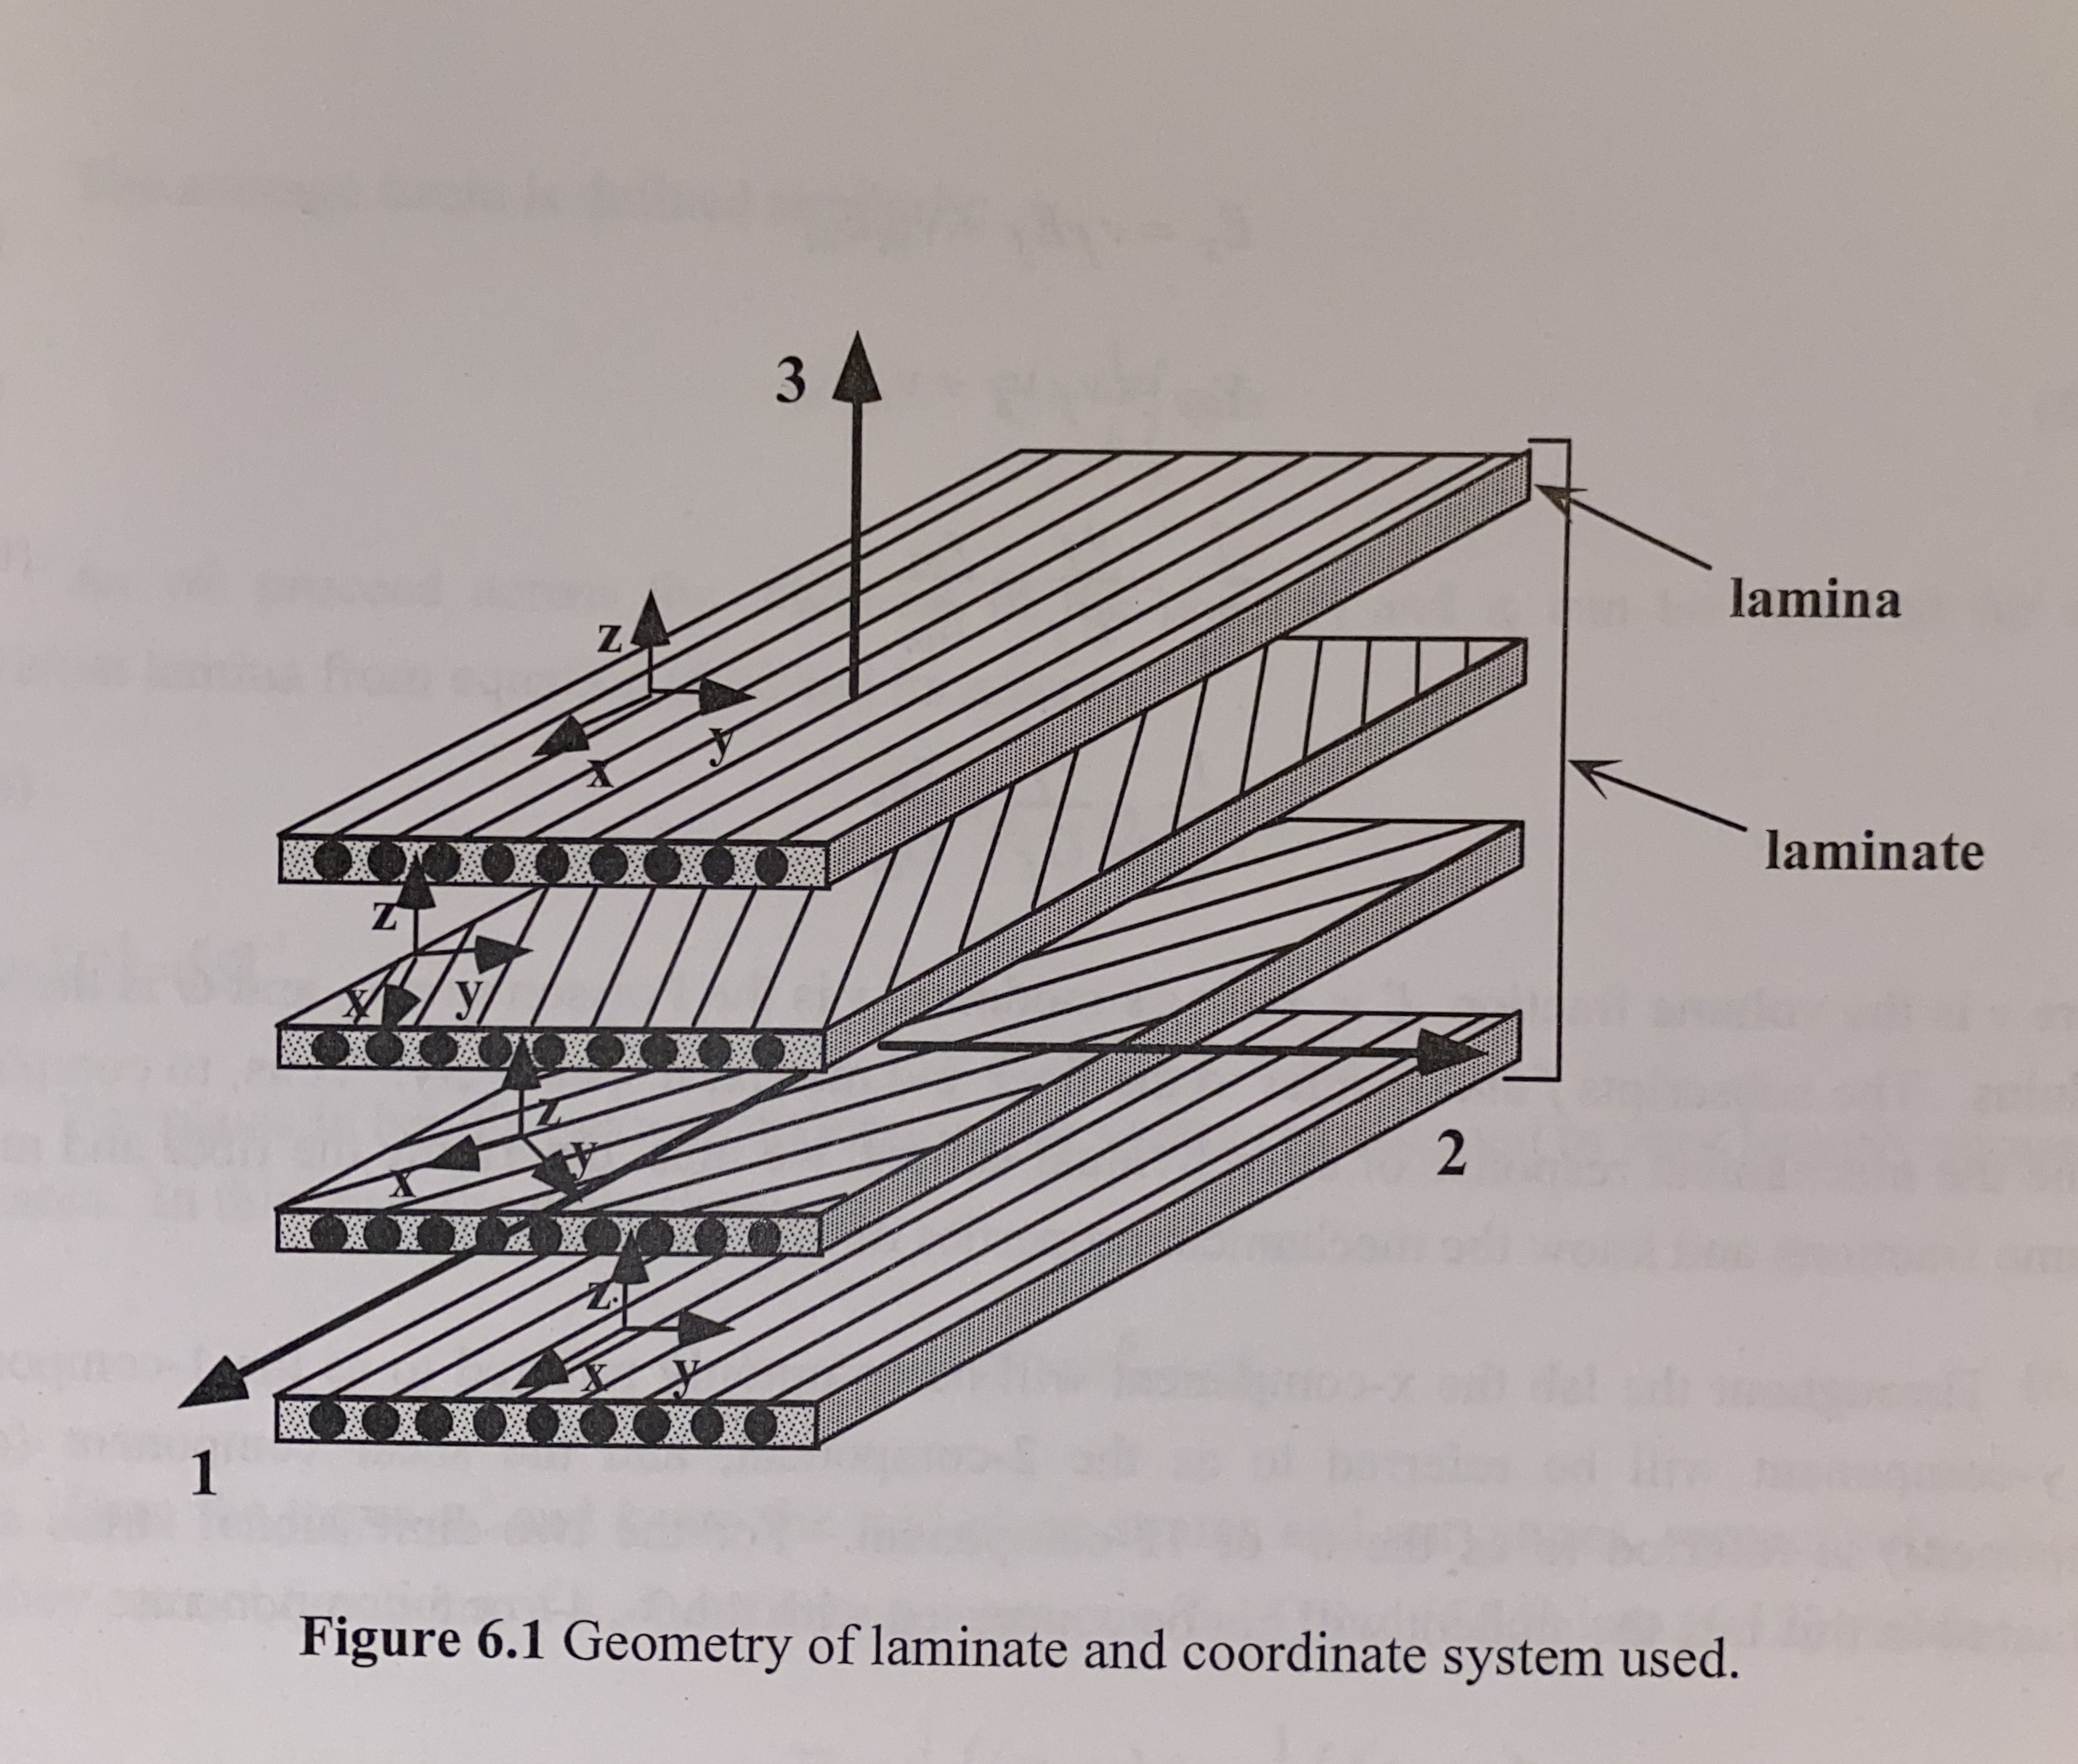
\includegraphics[width=0.45\textwidth]{Pictures/Theory and Analysis/coordsystem.jpg}
    \caption{Coordinate System\cite{labmanual}}
    \label{fig:coordsystem}
\end{figure}

Figure \ref{fig:coordsystem} shows the coordinate system used for analysis. Using this coordinate system and the assumption of plane stress, the only relevant stresses are $\sigma_1$ , $\sigma_2$, and $\sigma_6$. $\sigma_1$ and $\sigma_2$ correspond to the stresses in  x and y directions, while $\sigma_6$ corresponds to $xy$ shear stress. The stress-strain relationship is then:
\begin{equation}
    \epsilon_i = S_{ij}\sigma_j
\end{equation}
where $S_{ij}$ is the inverse of the previously mentioned stiffness matrix. For this case, we define $S_{ij}$ as:
\begin{equation}
    S_{ij} = 
    \begin{bmatrix}
    \frac{1}{E_x} & \frac{-\mbox{v}_{xy}}{E_x} & 0 \\
    \frac{-\mbox{v}_{xy}}{E_x} & \frac{1}{E_y} & 0 \\
    0 & 0 & \frac{1}{G_{xy}} 
    \end{bmatrix}
\end{equation}
where $E_x$ and $E_y$ are the longitudinal modulus and transverse modulus, $G_{xy}$ is the in-plane shear modulus, and v$_{xy}$ is the major Poisson's ratio. The stress-strain relationship for the lamina is now defined in terms of these constants. The values for these constants is estimated using the rule-of-mixtures (ROM). According to ROM, the constants can be calculated using the following equations.
\begin{equation}\label{eqn:eight}
    E_x = v_f E_f + v_mE_m
\end{equation}
\begin{equation} \label{eqn:nine}
    \mbox{v}_{xy} = v_f \mbox{v}_f + v_m \mbox{v}_m
\end{equation}
where $v$ is the volume fraction, $E$ represents Young's modulus, v represents Poisson's ratio, and G is the shear modulus. The stress-strain relationship for each lamina can now be calculated. Each individual lamina is stacked to form the laminate. It is then necessary to define the mechanical properties of the laminate in terms of the properties of each lamina layer. The laminates are modeled as plates, where the assumption of plane stress still holds. Thus, the relevant stresses are still $\sigma_1$, $\sigma_2$, and $\sigma_6$. The stress of the plate is then the average of the lamina stress values. 

\begin{equation}
    \overline{\sigma_{i}} = \frac{1}{h} \int_h \sigma_i dz
\end{equation}
Similarly for strain,

\begin{equation}
    \overline{\epsilon_{i}} = \frac{1}{h} \int_h \epsilon_i dz
\end{equation}
After evaluating the integration in these equations and substituting into the stress-strain relationship, the result is the following equation.

\begin{equation}
    \sigma_i = \frac{1}{h} A_{ij} \epsilon_{j}^{0} + \frac{1}{h} B_{ij} k_j
\end{equation}
where $A_{ij}$ is the laminate stiffness matrix and $B_{ij}$ is the coupling matrix.

\begin{equation}
    A_{ij} = \int_h Q_{ij}dz
\end{equation}
\begin{equation}
    B_{ij} = \int_h Q_{ij} z dz
\end{equation}
Because $Q_{ij}$ is constant woth respect ot the thickness of the ply, the expressions for $A_{ij}$ and $B_{ij}$ can be simplified.
\begin{equation}\label{eqn:15}
    A_{ij} = \sum_{k=1}^{N} (Q_{ij})_{k} (z_k - z_{k-1})
\end{equation}

\begin{equation}
    B_{ij} = \frac{1}{2} \sum_{k=1}^{N} (Q_{ij})_{k} (z_k^2 - z_{k-1}^2)
\end{equation}
Here, N is the number of plies and z is the distance from the midline to the $k^{th}$ ply. When a laminate is symmetric, the coupling matrix is eliminated. The resulting stress-strain relationship for a symmetric laminate is:
\begin{equation}
    \sigma_i = \frac{1}{h} A_{ij} \epsilon_{j}^{0}
\end{equation}

The in-plane stiffness matrix values are calculated using the following relationships:
\begin{equation} \label{eqn:18}
    \overline{Q}_{11} = cE_x
\end{equation}
\begin{equation}
    \overline{Q}_{22} = cE_y
\end{equation}
\begin{equation}
    \overline{Q}_{12} = c \mbox{v}_{xy} E_y
\end{equation}
\begin{equation}
    \overline{Q}_{66} = G_{xy}
\end{equation}
\begin{equation}\label{eqn:22}
    c = \left [1-\mbox{v}_{xy}^2 \frac{E_y}{E_x} \right]^{-1}
\end{equation}
Using the in-plane stiffness matrix, the off-axis stiffness matrix can be constructed.

After testing a composite laminate under uniaxial loading in a laboratory, the Young's modulus, shear modulus, and Poisson's ratio can be determined by analyzing the results. These constants can be predicted for comparison using the laminate stiffness matrix.
\begin{equation}
    E_1^0  = \frac{1}{a_{11}h}
\end{equation}
\begin{equation}
    E_2^0  = \frac{1}{a_{22}h}
\end{equation}
\begin{equation}
    \mbox{v}_{12}^0 = \frac{-a_{12}}{a_{11}}
\end{equation}
\begin{equation}
    G_6^0  = \frac{1}{a_{66}h}
\end{equation}
Note that a corresponds to the inverse of the laminate stiffness matrix ($A^{-1}$). 
\begin{comment}
Lastly, the failure properties of the material are considered. In this case, failure is defined using von Mises yield criterion. The yielding point occurs when distortion energy ($U_d$) reaches the following condition.

\begin{equation}
    U_d = \frac{1}{2G} J_2 = \frac{3}{4G} \tau_{oct}^2
\end{equation}
where $\tau_{oct}$ is the octahedral stress and $J_2$ is the second strain invariant. In the case of simple tension, $J_2$ for the yield point can be calculated as:

\begin{equation}
    J_2 = \frac{1}{3} \sigma^2
\end{equation}
\end{comment}
The von Misces and Tresca yield criterion are often used to investigate failure of isotropic materials, though analysis of failure of the composite laminate studied in this lab requires a more complicated approach. In this case, the quadratic polynomial failure theory is used. The primary equation used is:
\begin{equation}
    F_{ij} \sigma_{ij} \sigma_j + F_i \sigma_i = 1
\end{equation}
This equation defines the point at which failure will occur. $F_{ij}$ and $F_i$ are material parameters that characterize strength similarly to how yield strength corresponds to an isotropic material. The expressions to calculate these parameters are as follows:
\begin{equation}
    \overline{F}_{11} = \frac{1}{XX'}
\end{equation}
\begin{equation}
    \overline{F}_{22} = \frac{1}{YY'}
\end{equation}
\begin{equation}
    \overline{F}_{66} = \frac{1}{S^2}
\end{equation}
\begin{equation}
    \overline{F}_{12} = \frac{-1}{2}\sqrt{\overline{F}_{11} \overline{F}_{22}}
\end{equation}
\begin{equation}
    \overline{F}_{1} = \frac{1}{X} - \frac{1}{X'}
\end{equation}
\begin{equation}
    \overline{F}_{2} = \frac{1}{Y} - \frac{1}{Y'}
\end{equation}
Here, X and Y correspond to the longitudinal and transverse tension strength, while Y and Y' correspond to the longitudinal and transverse compression strength. S represents the in-plane shear stress. When considering the case of uniaxial tension, the quadratic polynomial failure equation becomes:

\begin{equation}
    F_{11} \sigma_{1}^2 + F_1 \sigma_1 = 1
\end{equation}







 % ----

\clearpage
\section{Apparatus} \label{sec:3}
\subsection{Apparatus for Manufacturing of Polymer Matrix Composites}
\tab A set DA 409U/G35 150 prepeg sheets were provided for the purposes of designing and forming both the $0\degree$ and $45\degree$ specimens.  A sharp utility knife was provided to slice the sheets into the proper dimensions.  Due to the high sensitivity to local humidity and temperature, the manufacturing process was done in a large, well ventilated room with an analog hygrometer/digital thermometer.  The analog hygrometer had a relative humidity accuracy of 2.5\% and resolution of 1.0\%; the digital thermometer had an accuracy of $1.5\degree$F and resolution of $0.1\degree$F.  For the purpose of weighing the specimen prior to cure, an electronic top loading balance scale was provided with a linearity of $\pm 0.001$ grams and $4.0$ second stabilization time.  During the measuring, cutting, and assembling of the specimen, slightly unconventional methods of chilling the composite were used to rapidly decrease the local temperature of the material to prevent premature curing and mitigate the slow increase of void content in the composite matrix.  Some methods included compressed air cans or thermal cold-sinks.  Additional information about the tools used in experiment six may be found in Table \ref{tab:equipmentpart1} below and labelled pictures displaying the components may be found in Figure \ref{fig:exp1}.

The lay-up portion of the lab primarily focused on setting the laminate within layers peel ply, bleeder ply, and release films.  Each of these layers served a purpose of absorbing, displacing, and stabilizing the resin during the thermosetting process.  The components used during the lay-up process are provided in Table \ref{tab:equipmentpart1} (\textit{continued}) and the pictures displayed in Figure \ref{fig:exp1b}.  Images were provided by the lab manual \cite{labmanual}, and included the key components for experiment 1.

\begin{table}[h!]
    \centering
    \caption{Equipment and Specifications for Specimen Manufacturing}
    \begin{tabular}{|c|C{0.25\textwidth}|C{0.25\textwidth}|C{0.12\textwidth}|C{0.2\textwidth}|}\toprule
        \textbf{No.} & \textbf{Item} & \textbf{Description} & \textbf{Accuracy} & \textbf{Use in Experiment} \\ \midrule
        \textbf{1} & DA 409U/G35\newline 150 prepreg & Unidirectional reinforcement,\newline G35 graphite fibers,\newline 409 epoxy matrix, Prepreg planar density of $\rho = 150 g/m^2$ & N/A & Slices were cut out of preform sheets to construct polymer composite specimen \\ \hline
        \textbf{2} & Traceable\textsuperscript{\tiny\textregistered} Analog Hygrometer/ \newline Digital Thermometer & 5.0 inch dial,\newline RH range: 0\% - 100\%.\newline Thermometer range: $23.0\degree-131.0\degree$F & RH $2.5\%$, T $1.5\degree$F & Placed in layup, weighing, and hot press rooms. \\\hline
        \textbf{3} & Electronic Top Loading Balance & Highly sensitive scale & $\pm0.001$ g & Weigh composite specimen \& bleeder cloth before and after cure \\\hline
        \textbf{4} & Carver Programmable Hot press & Electrical Platens,\newline Max Temperature $850\degree$F,\newline Max Pressure 24 tons & N/A & Hot press to thermoset the composite \\\hline
    \end{tabular}
    \label{tab:equipmentpart1}
\end{table}

\begin{table}[h!]
    \centering
    \begin{tabular}{|c|C{0.25\textwidth}|C{0.25\textwidth}|C{0.12\textwidth}|C{0.2\textwidth}|}
        \multicolumn{5}{c}{\textbf{Table 1} (\textit{continued})\textbf{:} \textbf{Lay-up Materials}} \\\midrule
        \textbf{5} & AirTech N10 Bleeder Cloth & Absorb excess resin \& \newline Provide vacuum path to remove volatiles & N/A & Bleeder cloth to absorb resin \\\hline
        \textbf{6} & Release-Ease 234 TFP Peel Ply & Teflon coated to prevent resin sticking & N/A & Porosity allowed uniform displacement of resin while preventing undesired adhesion \\\hline
        \textbf{7} & A4000R Non-perforated TFP Film & Placed between press and layup materials & N/A & Prevents lay-up materials from adhering to the mold and tool \\\hline
        \textbf{8} & 2024-T3 Aluminium Mold & Three $1.0 x 7.0$ slots for lay-up material & N/A & Holds the lay-up material while placed in hot press \\\bottomrule
    \end{tabular}
\end{table}

\begin{figure}[!h]
  \begin{subfigure}[t]{.4\textwidth}
    \centering
    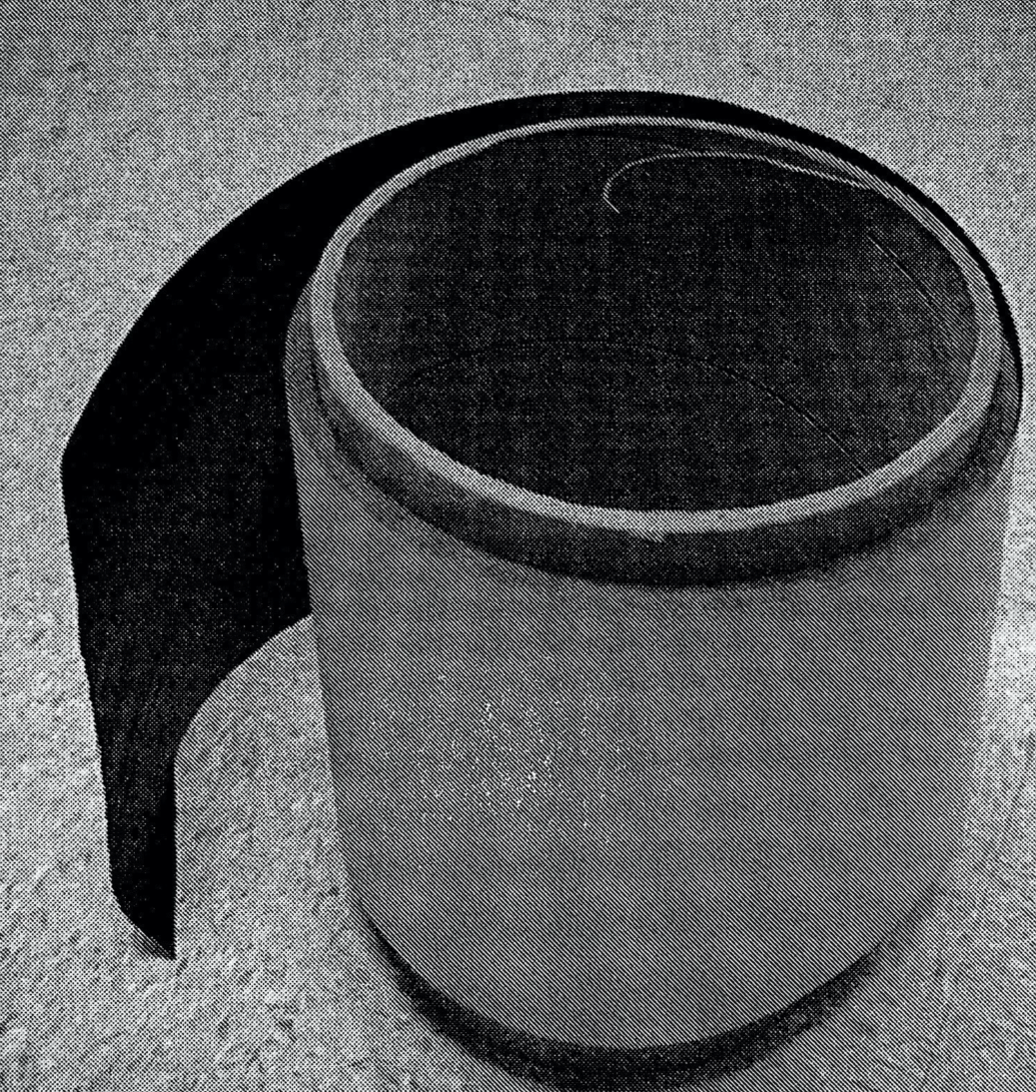
\includegraphics[width=\linewidth]{Pictures/Apparatus/Experiment 1/one.png}
    \caption{\textbf{1.} DA 409U/G35 150 prepreg}
  \end{subfigure}
  \hfill
  \begin{subfigure}[t]{.4\textwidth}
    \centering
    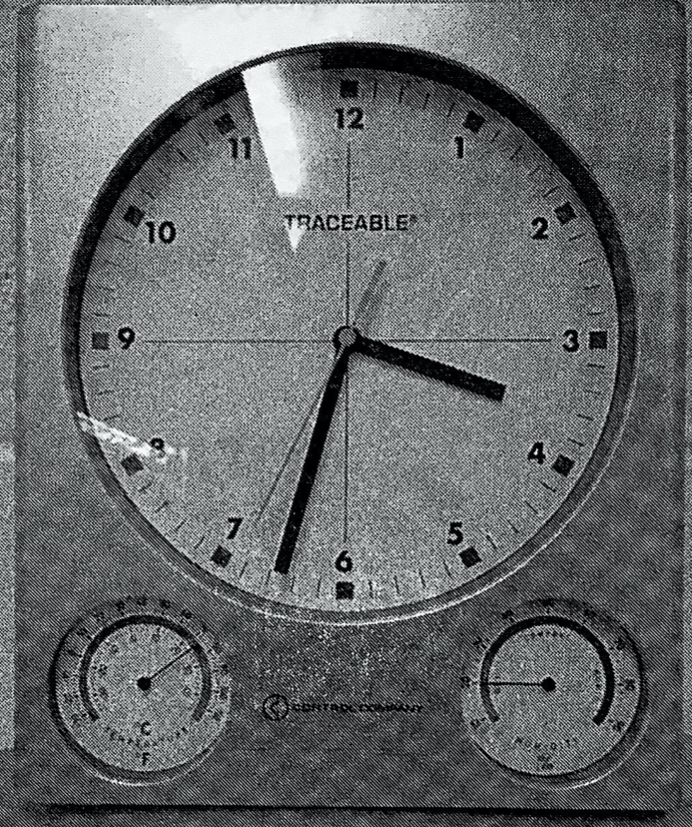
\includegraphics[width=\linewidth]{Pictures/Apparatus/Experiment 1/two.png}
    \caption{\textbf{2.} Analog Hygrometer/Digital Thermometer}
  \end{subfigure}

  \medskip

  \begin{subfigure}[t]{.4\textwidth}
    \centering
    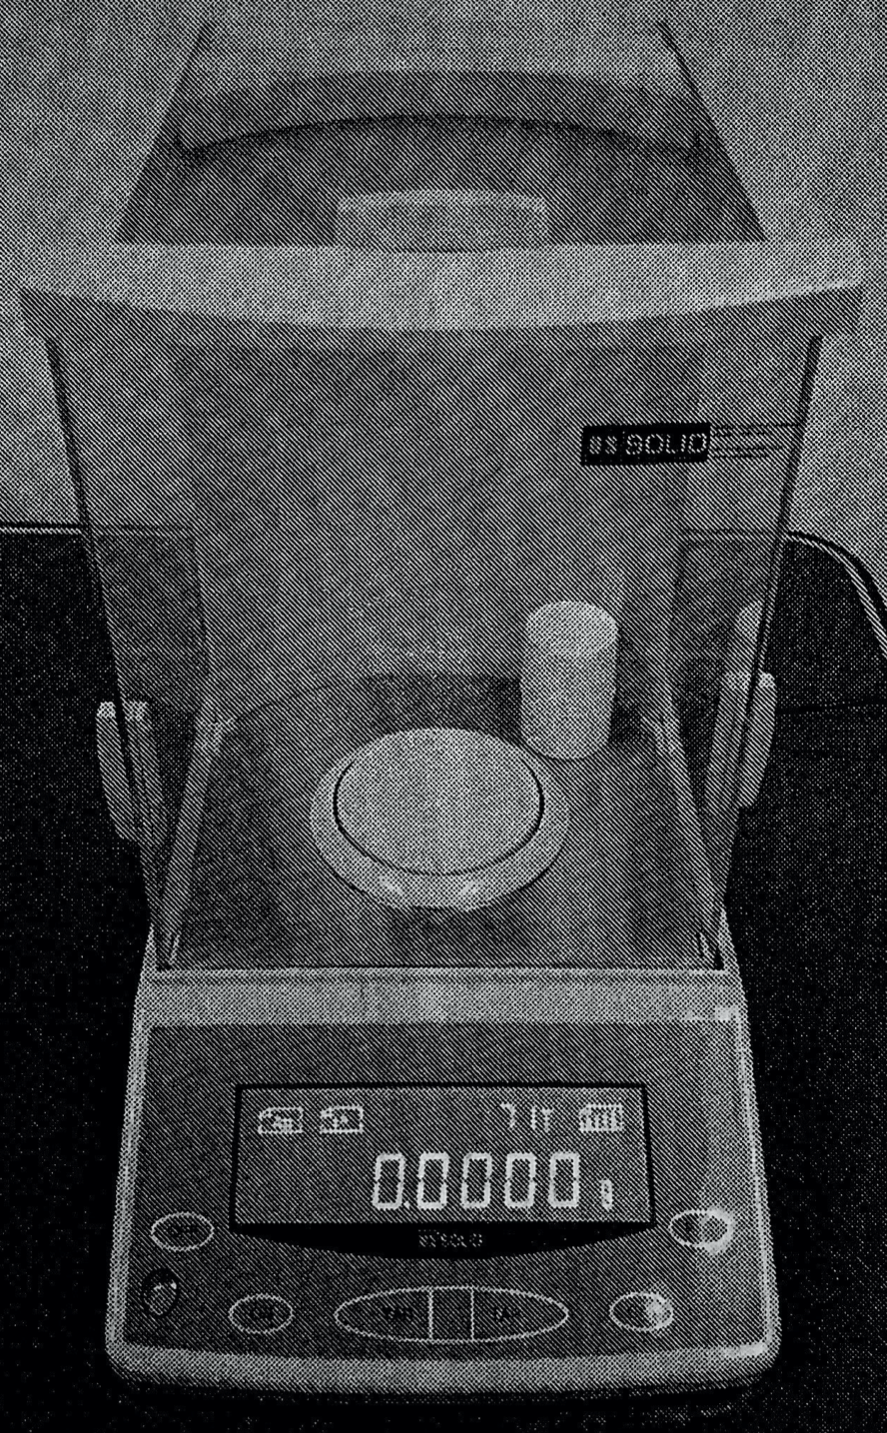
\includegraphics[width=\linewidth]{Pictures/Apparatus/Experiment 1/three.png}
    \caption{\textbf{3.} Electronic Top Loading Balance}
  \end{subfigure}
  \hfill
  \begin{subfigure}[t]{.4\textwidth}
    \centering
    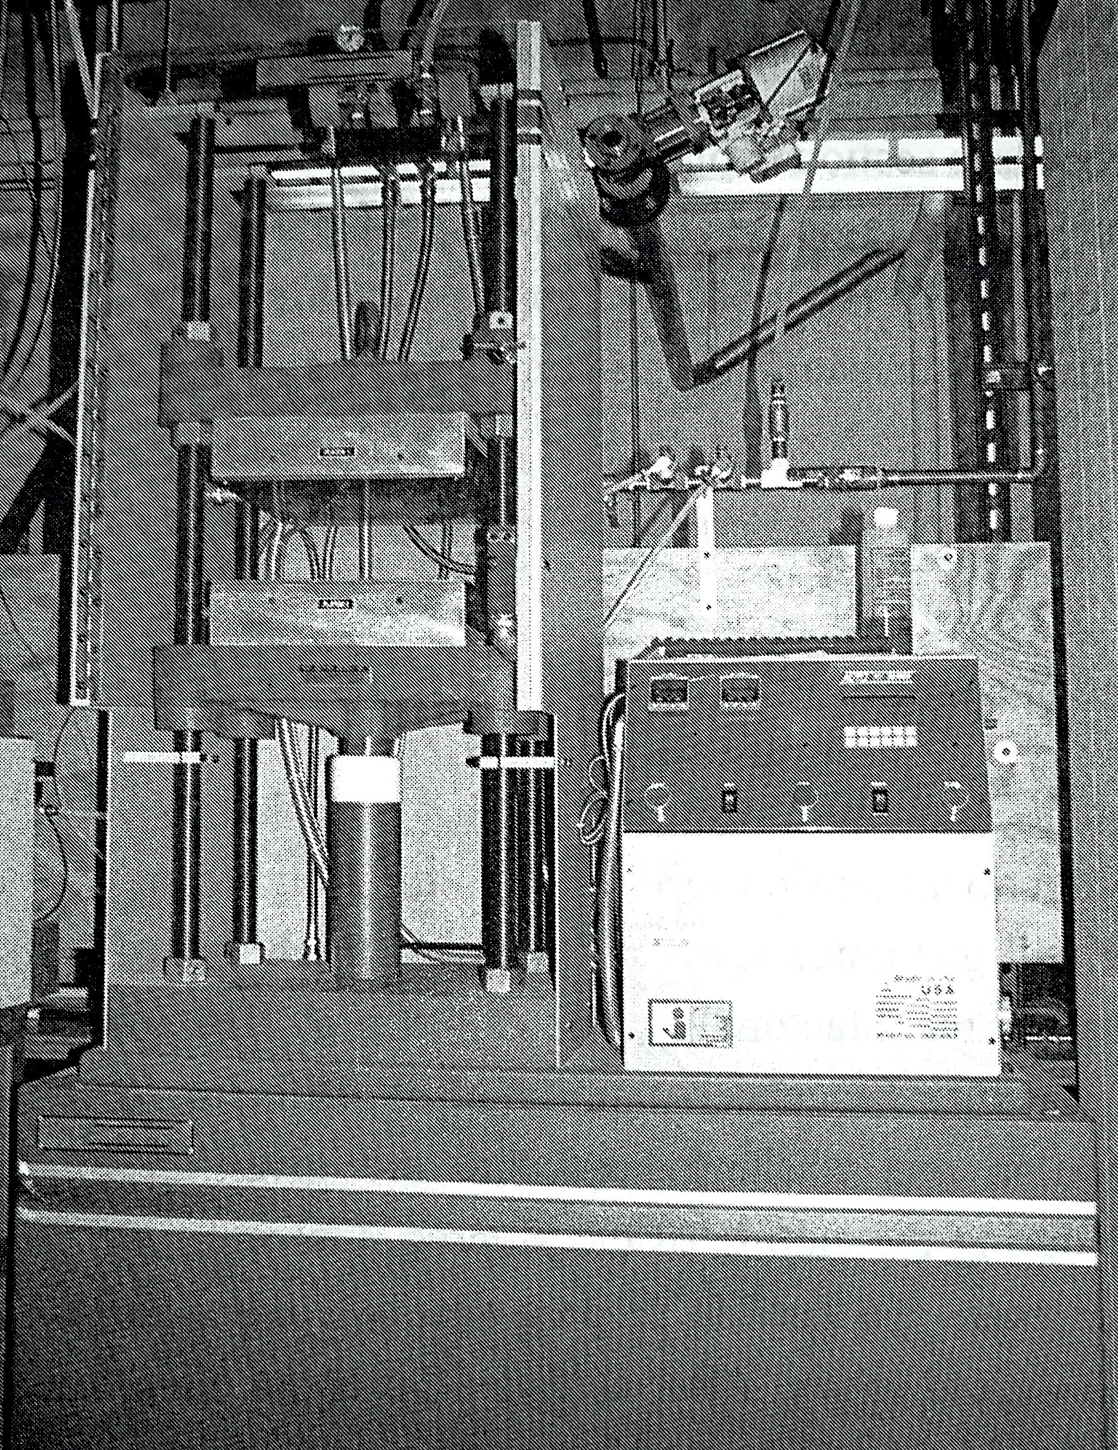
\includegraphics[width=\linewidth]{Pictures/Apparatus/Experiment 1/eight.png}
    \caption{\textbf{4.} Carver Programmable Hot Press}
  \end{subfigure}
  \caption{Experiment 1 Assembly Tools}
  \label{fig:exp1}
\end{figure}

\clearpage

\begin{figure}[!h]
  \begin{subfigure}[t]{.4\textwidth}
    \centering
    
\includegraphics[width=\linewidth]{Pictures/Apparatus/Experiment 1/four.png}
    \caption{\textbf{5.} AirTech N10 Bleeder Cloth}
  \end{subfigure}
  \hfill
  \begin{subfigure}[t]{.4\textwidth}
    \centering
    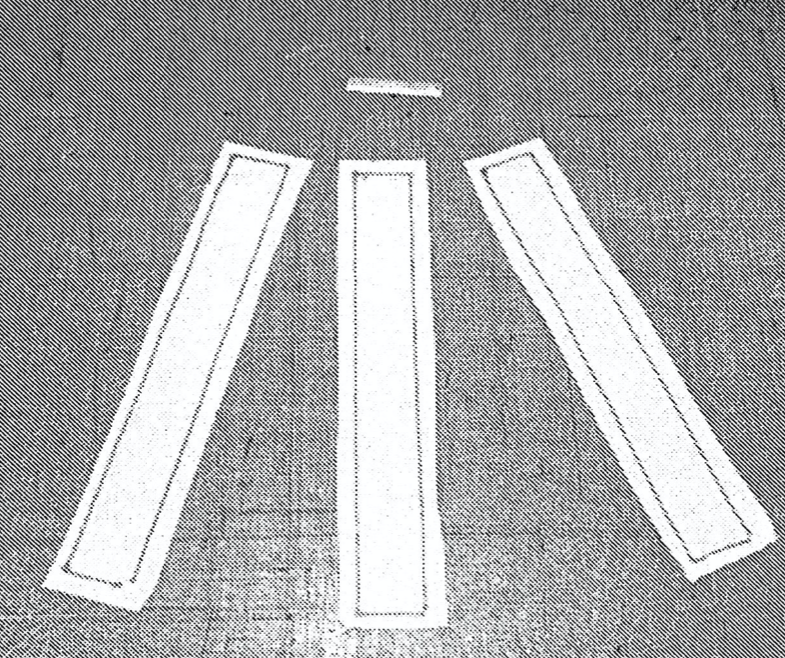
\includegraphics[width=\linewidth]{Pictures/Apparatus/Experiment 1/five.png}
    \caption{\textbf{6.} Release-Ease 234 TFP Peel Ply}
  \end{subfigure}

  \medskip

  \begin{subfigure}[t]{.4\textwidth}
    \centering
    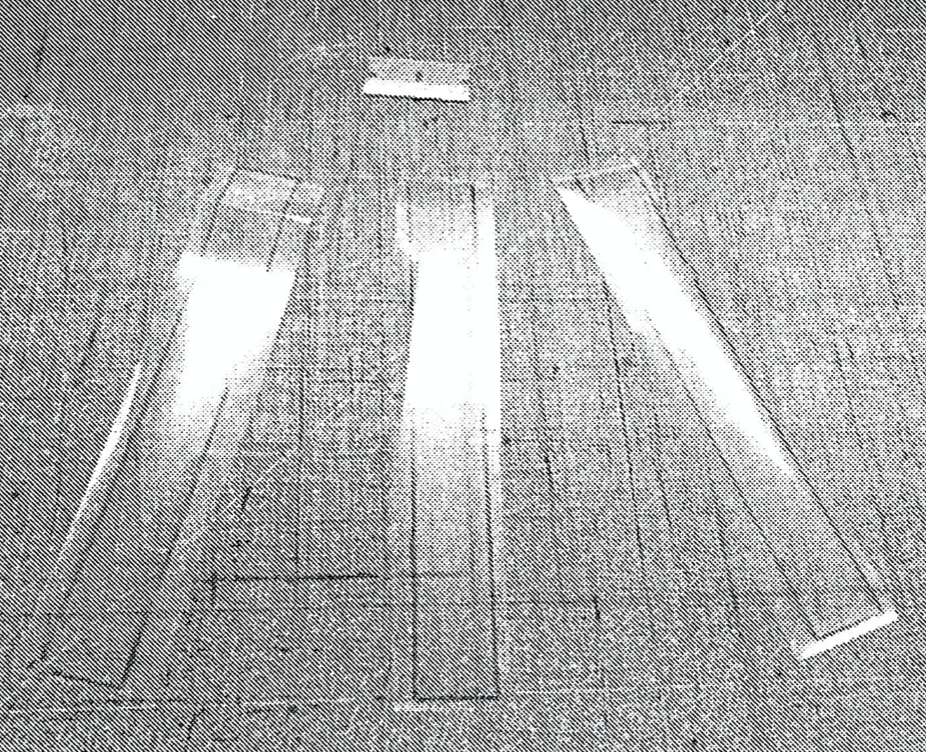
\includegraphics[width=\linewidth]{Pictures/Apparatus/Experiment 1/six.png}
    \caption{\textbf{7.} A4000R Non-perforated TFP Film}
  \end{subfigure}
  \hfill
  \begin{subfigure}[t]{.4\textwidth}
    \centering
    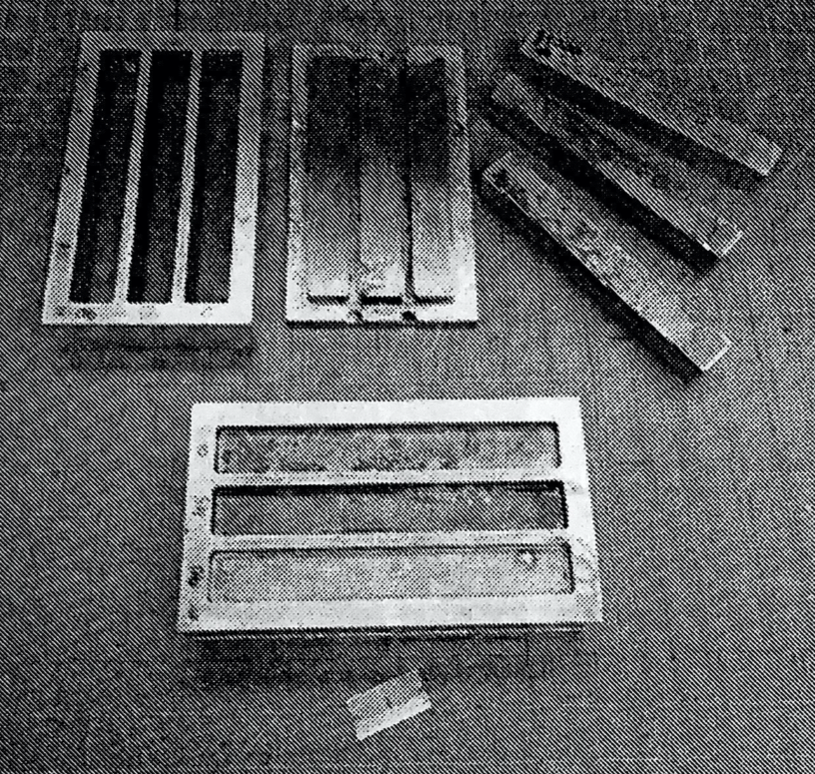
\includegraphics[width=\linewidth]{Pictures/Apparatus/Experiment 1/seven.png}
    \caption{\textbf{8.} 2024-T3 Aluminium Mold}
  \end{subfigure}
  \caption{Experiment 1 Lay-up Tools}
  \label{fig:exp1b}
\end{figure}

\clearpage

\subsection{Apparatus for Mechanical Property Testing of Composite Materials}
\tab Experiment 6 focused on testing the composite specimen created in experiment 1.  To determine the mechanical properties of the composite materials, the specimen were loaded with tension using the Instron model 4483, screw-driven machine.  The Instron 4483 has a load cell to measure the force exerted on the specimen.  In addition, the strain was measured using the Instron 2630-100 static extensometer, which observes the strain of the specimen with an electrical calibration accuracy (ECA) of approximately $\pm0.06$ full range output (FRO).  The two devices, connected to a laboratory computer to record data, were used to test the three specimen.  Additional information about the apparatus used in experiment six may be found in Table \ref{tab:equipmentpart3} below and labelled pictures displaying the components may be found in Figure \ref{fig:exp6}.

\begin{table}[h!]
    \centering
    \caption{Equipment and Specifications for Uniaxial Tension Testing}
    \begin{tabular}{|c|C{0.25\textwidth}|C{0.25\textwidth}|C{0.12\textwidth}|C{0.2\textwidth}|}\toprule
        \textbf{No.} & \textbf{Item} & \textbf{Description} & \textbf{Accuracy} & \textbf{Use in Experiment} \\ \midrule
        \textbf{1} & Instron model 4483 & Screw-driven tension compression tests\newline Max load 20 kips & N/A & Used to exert tension load on specimen \\\hline
        \textbf{2} & Instron model 2630-100 static Extensometer & 1.0 inch gauge length & ECA:\newline $\pm0.06$ FRO \cite{extensometer} & Measure specimen strain \\\hline
    \end{tabular}
    \label{tab:equipmentpart3}
\end{table}

\hl{ADD PICTURES} % ----

\clearpage
\section{Procedure} \label{sec:4}
\subsection{Process for Manufacturing of Polymer Matrix Composites}
\subsubsection{Assembly of Laminate}


\subsubsection{Lay-up Procedure}


\subsubsection{Thermosetting Procedure}



\subsection{Process for Mechanical Property Testing of Composite Materials}
\subsubsection{Specimen Geometry}


\subsubsection{Tension Test} % ----

\clearpage
\section{Experimental Uncertainty} \label{sec:5}
Sources of uncertainty in this experiment consist of the measurement devices used and calculated quantities presented. In the case of measured values, the uncertainty is an estimate of the instrument using the experiment data given. For calculations, the method of uncertainty propagation is used to find the uncertainty of each variable. Zero uncertainty is assumed for material properties given in the lab manual. Since uncertainty in this experiment is due to the devices used to gather data, increasing the accuracy of the measurement instruments will reduce the uncertainty. User error can be lowered as well by taking repeated measurements, such as when finding specimen dimensions or mass. Sample calculations of uncertainty propagation are documented in the Appendix C.       
\begin{table}[!h]
    \centering
    \caption{Uncertainty \cite{labmanual}}
    \begin{tabular}{|c|c|c|}\toprule
        \multicolumn{3}{c}{\textbf{Uncertainty Estimation}} \\ \midrule
        \textbf{Data} & \textbf{Uncertainty} & \textbf{Reasoning} \\ \hline\hline
        Load                        & 0.00005 N  & Estimate of measurement device \\\hline
        Specimen Length         & 0.00005 m  & Estimate of measurement device  \\\hline
        Specimen Width         & 0.00000005 m  & Estimate of measurement device  \\\hline
        Specimen Thickness         & 0.00000005 m  & Estimate of measurement device  \\\hline
        Specimen Mass             &  0.00005 kg & Estimate of measurement device\\\hline
        Strain Extensometer         & 0.00005 & Estimate of measurement device  \\\hline
        Strain DIC                  & 0.00005 & Estimate of measurement device  \\\hline
        Specimen Density            & 8.065 e-9 kg/m$^3$ & Calculated using uncertainty propagation  \\\hline
        Specimen Volume             & 0.0018 m$^3$ & Calculated using uncertainty propagation  \\\hline
        Specimen Volume Shrinkage   & 0.0255 m$^3$ & Calculated using uncertainty propagation  \\\hline
        Elastic Modulus             &  & Calculated using uncertainty propagation  \\\hline
        $E_{x}$                     &  & Calculated using uncertainty propagation  \\\hline
        $\nu_{xy}$                  &  & Calculated using uncertainty propagation  \\\hline
        $E_{y}$                     &  & Calculated using uncertainty propagation  \\\hline
        $G_{xy}$                    &  & Calculated using uncertainty propagation  \\\hline
        %$c$                         &  & Calculated using uncertainty propagation  \\\hline
        %$\overline{Q}_{11}$         &  & Calculated using uncertainty propagation\\\hline      
        %$\overline{Q}_{22}$         &  & Calculated using uncertainty propagation\\\hline                        
        %$\overline{Q}_{12}$         &  & Calculated using uncertainty propagation\\\hline                        
        %$\overline{Q}_{66}$         &  & Calculated using uncertainty propagation\\\hline               
        %${Q}_{16}$                  &  & Calculated using uncertainty propagation\\\hline                        
        %${Q}_{26}$                  &  & Calculated using uncertainty propagation\\\hline                        
        Theoretical Failure Load    & 0 Pa & Calculated using uncertainty propagation\\\hline                        
        %    & & \\\hline                        
         %   & & \\\hline                        
          %  & & \\\hline                   
        Lab Relative Humidity       & 0.1$\%$ & Estimate of measurement device    \\\hline
        Lab Temperature             & 0.1$\degree$ & Estimate of measurement device   \\\bottomrule
    \end{tabular}
    \label{tab:uncertainty}
\end{table} % ----

\clearpage
\section{Results and Discussion} \label{sec:6}
% Experiment 1
\subsection{}
% Tabulate all data, experimental and calculated, and include them in your report (combined with lab assignment #6)


\subsection{}
% Determine the average composite density before and after cure, along with the standard deviation.  What is the average uncured thickness of each composite ply?  What is the average cured thickness of each composite ply?  How does this compare to the specifications in Table 1.2 for this composite system (for the cured ply only)?

Based on the dimensions and mass from Table \ref{tab:beforedimensions}, the densities of each specimen was tabulated in Table \ref{tab:beforedensity} assuming each specimen is a rectangular prism. The average densities and standard deviation for both uncured and cured specimens are shown as well. Table \ref{tab:ply_thickness} shows the thickness of each composite ply, where 16 plies were used to construct specimens a and b, and 8 plies were used for specimen c. This was compared to the datasheet provided from Table 1.2 in the lab manual \cite{labmanual}.

\begin{table}[!h]
    \centering
    \caption{Composite Densities}
    \begin{tabular}{|l||c|c|}\toprule
        Specimen & Uncured Density & Cured Density \\ 
        & (\textit{g / cm$^{3}$}) & (\textit{g / cm$^{3}$}) \\ \midrule
        \textbf{(a)}: $[90\degree]_{16\text{T}}$  & 1.4739 & 1.5691 \\\hline
        \textbf{(b)}: $[\pm45\degree_4]_{2\text{S}}$ & 1.4656  & 1.5667 \\\hline
        \textbf{(c)}: $[0\degree]_{8\text{T}}$ & 1.4716 & 1.5726 \\\bottomrule
        Average & 1.4703 & 1.5695 \\\hline
        Standard Deviation & 0.0043 & 0.0030 \\\bottomrule
    \end{tabular}
    \label{tab:beforedensity}
\end{table}

\begin{table}[!h]
    \centering
    \caption{Ply Thickness}
    \begin{tabular}{|l||c|c|c|}\toprule
        Specimen & Uncured Thickness & Cured Thickness & Cured Thickness \\
        & (\textit{mm}) & (\textit{mm}) & Datasheet (\textit{mm}) \\ \midrule
        \textbf{(a)}: $[90\degree]_{16\text{T}}$  & 0.1647 & 0.1383 & 0.1524 \\\hline
        \textbf{(b)}: $[\pm45\degree_4]_{2\text{S}}$ & 0.2162 & 0.1584 & 0.1524 \\\hline
        \textbf{(c)}: $[0\degree]_{8\text{T}}$ & 0.2414 & 0.1936 & 0.1524 \\\bottomrule
        Average & 0.2074 & 0.1634 & 0.1524 \\\bottomrule
    \end{tabular}
    \label{tab:ply_thickness}
\end{table}

The average cured densities for all specimens was 1.5695 g/cm$^{3}$. The datasheet predicts the average cured density for this composite should be approximately 1.53 g/cm$^{3}$. The percent difference between the experimental specimens and the datasheet density is 2.58\%, which is very similar. On the other hand, there appears to be a higher deviation between the datasheet and experimental ply thickness. The average experimental cured ply thickness was 0.1632 mm while the data sheet states the cured ply thickness is 0.1524 mm, or a 7.21\% difference. While this is fairly close to the data sheet, there are still possible explanations for this discrepancy. One possible source of this error could be manufacturing precision. Considering the specimens were constructed by hand with simple tools (scissors and rulers) and are not dimensionally exactly the same as its mold, it is likely these specimens are not constructed up to ideal specifications. For example, a varying amount of residual resin or voids could be in between each fiber, changing the distance between each ply, thus varying the ply thickness.   


\subsection{}
% Using the data in Table 1.2 and question (1), and assuming zero voids in the specimens, determine the fiber volume fraction for the composite before and after cure in each specimen.  How does the cured composite fiber volume fraction compare to the material specifications?  What are possible sources of error?


\subsection{}
% What is the total volumetric shrinkage of each composite specimen after cure?  How does this compare to the materials specification data?

Based on the dimensions of the specimen before and after curing, the volumetric shrinkage was calculated with Equation \ref{eq:volume_shrinkage}. The $V_\text{uncured}$ and $V_\text{cured}$ terms represent the volume of the specimen, uncured and cured, respectively. The shrinkage values for each specimen is shown in Table \ref{tab:volume_shrinkage_tab}. 

\begin{equation} \label{eq:volume_shrinkage}
    \% \text{Shrinkage} = \frac{V_\text{uncured} - V_\text{cured}}{V_\text{cured}} * 100 \%
\end{equation}


\begin{table}[!h]
    \centering
    \caption{Volumetric Shrinkage}
    \begin{tabular}{|l||c|c|c|}\toprule
        Specimen & Uncured Volume & Cured Volume & Shrinkage \\ 
        & (\textit{cm$^{3}$}) & (\textit{cm$^{3}$}) & (\%) \\ \midrule
        \textbf{(a)}: $[90\degree]_{16\text{T}}$ & 11.65 & 8.74 & 33.28 \\\hline
        \textbf{(b)}: $[\pm45\degree_4]_{2\text{S}}$ & 14.45 & 10.81 & 33.63 \\\hline
        \textbf{(c)}: $[0\degree]_{8\text{T}}$ & 8.28 & 6.21 & 33.40 \\\bottomrule
    \end{tabular}
    \label{tab:volume_shrinkage_tab}
\end{table}

Based on the lab manual, from Table 1.2 in Appendix G, the volumetric shrinkage is expected to be 70\%. However, from Table \ref{tab:volume_shrinkage_tab}, the experimental shrinkage was only about 33\%. Again, this is likely due to poor manufacturing tolerances. This also lines up with the theory that there are more voids or excess resin left in the composite, thus increasing the specimens' final volume and decreasing its shrinkage percentages.

\subsection{}
% Calculate the force needed to be applied by the hot press platens to achieve 150 psi on the specimens.

In order to achieve 150 psi of pressure on the specimen, the hot press must apply a total of at least 1,050 lbf. Each specimen is 1x7 inches. By distributing the pressure evenly to all 7 sq inches, 1,050 lbf is needed. However, note that the force required is likely slightly higher since this calculation assumes the total contact area is exactly the same area as the specimen area. In reality, given all the mounting hardware and mold, the contact area must be higher than the specimen size.


\subsection{}
% Comment on the quality of the manufactured specimens.  (Where there any problems during lay-up or cure which may impact the mechanical performance?)
In an ordinary semester, without the Covid-19 quarantine situation, the specimen would be removed from their molds after curing and the condition observed.  Due to state-wide shutdown, it was not possible for students to physically retrieve the specimen and observe its condition.  According to an email from Professor Ioannis Chasiotis, dated May 8, 2020, the thickness of the specimen decreased.  With this observation, the only inference possible without physical observation is that the platens have sunk deeper into the mold following the curing process.

\subsection{}
% What would happen if the cure temperature was raised to a higher temperature?  How about a lower temperature?
\tab The DA 409U/G35 150 prepreg used in this experiment requires temperature cure to properly complete the manufacturing process and create the epoxy cross-links.  The temperature curing process, a process henceforth defined as thermosetting, is a very critical stage wherein temperature and pressure is applied to the specimen through a hot press to begin the polymerization, or cross-linking of the resin matrix.  In this experiment, a prepreg was used to form the specimen, which is useful for generating small, thin-skinned specimen for testing or thin walled applications, but is prone to premature curing depending on the local room temperature.

During the assembling process (\textit{lay-up stage}) of the composite specimen, an observation was made such that the curing process was able to begin prematurely due to the local heat generated by physical touch.  The lab manual warned of consequences directly linked to premature curing such as reduced mechanical quality due to malformed epoxy cross-links.  As such, rapid freezing or chilling techniques using condensed air or placement near a cold thermal-sink were applied to mitigate premature cure.  When the specimen were fully assembled, they were placed into molds (\textit{pre-cure stage}) with peeler ply, release film, and bleeder cloths.  When completed, the composites were ready for the thermosetting process.

\newpage
It is important to note that the temperature setting for the curing stage was controlled by the teaching assistants; and, variation of the curing temperature was not a focus of this experiment.  The temperature and pressure applied for the curing process was selected and performed according to the Carver programmable hot press with a cure cycle programmed by the lab staff.  If the temperature were to increase, the development of the cross-links would be much faster and rapid, which may improve the cure by preventing resin bleed and higher shrinkage would occur.  Higher shrinkage, depending on the application, may be desired due to the improvement in the material's thermal and electrical conductivity \cite{curematters}.  Higher temperature is not always good, though, as excessive temperature can result in a severe degradation of resin matrix.\cite{boeingcuring}  A lower temperature setting for the cure process of the specimen might result in the desired design performance due to a lower setting of the cross-link structures.  Variation of curing temperature may result in a variation in the quality of the cross-link structures, resin leakage, or material shrinkage.

\subsection{}
% What would happen if the applied pressure was raised to a higher pressure? How about a lower pressure?

\subsection{}
% Include the average room temperature and humidity during lay-up.  Would the quality of the manufactured specimens be affected by the room temperature and humidity levels?  Explain.

The lab group did not record the average room temperature and humidity readings during the lay-up process. Thus, we presume that the the lay-up process was completed under standard lab conditions: 23$\degree$C and 40\% relative humidity. Room temperature and humidity levels are influential on the quality of manufactured specimens. During storage, the composite prepreg is kept at freezing temperatures. As the temperature increases, the epoxy will begin to crosslink. While this behavior is desired during the curing process, it is important to to avoid curing the composites prematurely from a high room temperature. Note that premature crosslinking reduces the quality of the composite specimen. It is also important to regulate the humidity level during the layup process to prevent the specimen from absorbing additional moisture. Moisture absorption can lead to the formation of more voids, which are unfilled pores in the specimen. These voids are major manufacturing defects that reduce the performance of the specimen in terms of mechanical properties and lifespan.

\subsection{}
% Include the temperature and pressure history of the cure cycle in the report.
After the layup phase is completed, the curing process can begin. In general, the curing process involves exposing the specimen to high temperatures and pressures. Both the magnitude and duration of the elevated temperatures and pressures influence the quality of the final specimen. Different materials require different cure cycle characteristics for optimal results. A typical cure cycle can be divided in two major steps: the consolidation stage and the cure stage. During the consolidation stage, heat is applied to reach an intermediate temperature and pressure is applied. The heat reduces the viscosity of the resin and the pressure squeezes excess resin out of the laminate. The pressure also "consolidates" the individual specimen plies and removes voids.  During the cure stage, the temperature is elevated even more. The higher temperature initiates resin polymerization and produces cross-linking. 

\begin{figure}[H]
    \centering
    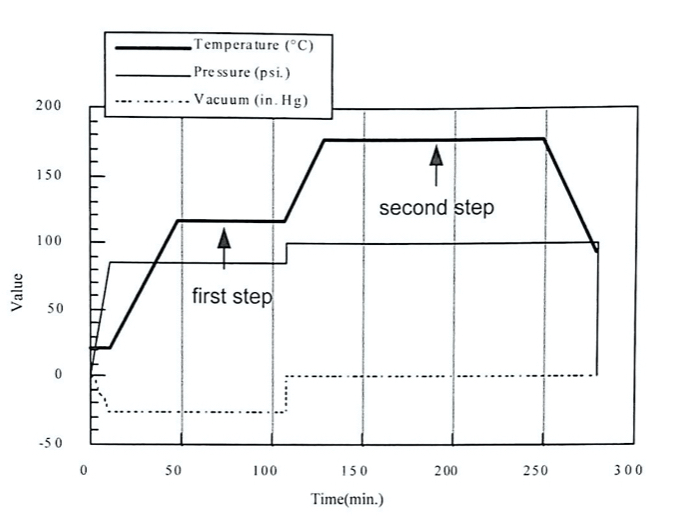
\includegraphics[width=0.8\textwidth]{Pictures/Lab1: Q 1.10/typical_cure.jpg}
    \caption{Typical Cure Cycle\cite{labmanual}}
    \label{fig:typicalcure}
\end{figure}

Figure \ref{fig:typicalcure} displays the temperatures and pressures in a typical cure cycle. Here, the difference in temperatures and pressures between the first and second steps can be seen. Note that this figure corresponds to a typical cure cycle, and not the one used for this lab.

For this lab, a single step cure cycle is used. In this case, the temperature and pressure are raised to a predetermined value only once. Figure \ref{fig:mariecuring} displays the curing cycle for the specimen used in this lab. The single step, as opposed to two steps in the cycle discussed earlier, can be seen in this figure.



\subsection{}
% Explain why the heating rate is much more linear than the cooling rate.

The curing cycle involves a rise in temperature for polymerization and then a cooling period afterwards. The temperatures that the specimen experiences during the cycle are determined by the hot press platens. It is important to note that the platens do not heat and cool at the same rate. The heating rate is much more linear than the cooling rate, which can be attributed to the processes by which the platens are heated and cooled. The heating rate is controlled through a process known as Joule heating. In this process, an electrical current is passed through a conductor, which produces heat. The heating rate can then be monitored using a thermocouple and actively controlled through the electric current. In contrast, the platens are cooled using flowing chilled water. In this case, not only is the cooling rate not actively controlled, but the flow rate is also constant. The cooling rate of the platens slows down over time since the temperature of the platens decreases, while the temperature of the chilled flowing water is constant. This results in a nonlinear cooling rate.

\subsection{}
% When does compaction of the composite laminate take place during the cure cycle? (Hint: When does the platen height change dramatically during the cure cycle?)


\clearpage

% Experiment 6
% \setcounter{subsection}{0}
\subsection{}
% Plot the stress versus strain curves for each test using the strain from the digital extensometer and the DIC calculations (i.e. two curves for each specimen).  Plot both stress vs strain curves for each specimen in the same plot.

In order to get an accurate idea of how these materials behaved and the mechanical properties of each layup, a stress vs. strain graph is a very useful tool. In this experiment the strain on each specimen was measured using two different methods, a digital image correlation (DIC) and the Instrom 2630-100 digital extensometer. This allowed for more accurate measurements to be taken and then compared once the experiment was finished. Although, there was an offset from between the DIC and extensometer, so that had to be corrected in the data before an accurate comparison could take place. With information on the strain, load, and size of each specimen, the following figures could be created for the $0\degree$, $45\degree$, and $90\degree$ laminates shown in Fig \ref{fig:stressvsstrain}.  One interesting to note from this is the behavior before breaking of all three tests. It can be seen in Fig \ref{fig:0lam} and Fig \ref{fig:90lam} that the stress is fairly linear until there is a sudden catastrophic failure with very little deformation of the material. This has to do with the orientation of the ply's within the composite, and when the are either parallel or perpendicular to the force, this type of behavior is to be expected. In Fig \ref{fig:45lam}, there is a linear region that translates to a more shallow slope until failure. This type of behavior occurs again due to the orientation of the laminates, with the load being distributed through both the matrix and fibers of the composite resulting in greater deformation and changes in the material property before failure. 

\begin{figure}[!h]
    \begin{center}
    \begin{subfigure}[b]{0.45\linewidth}
        \centering
        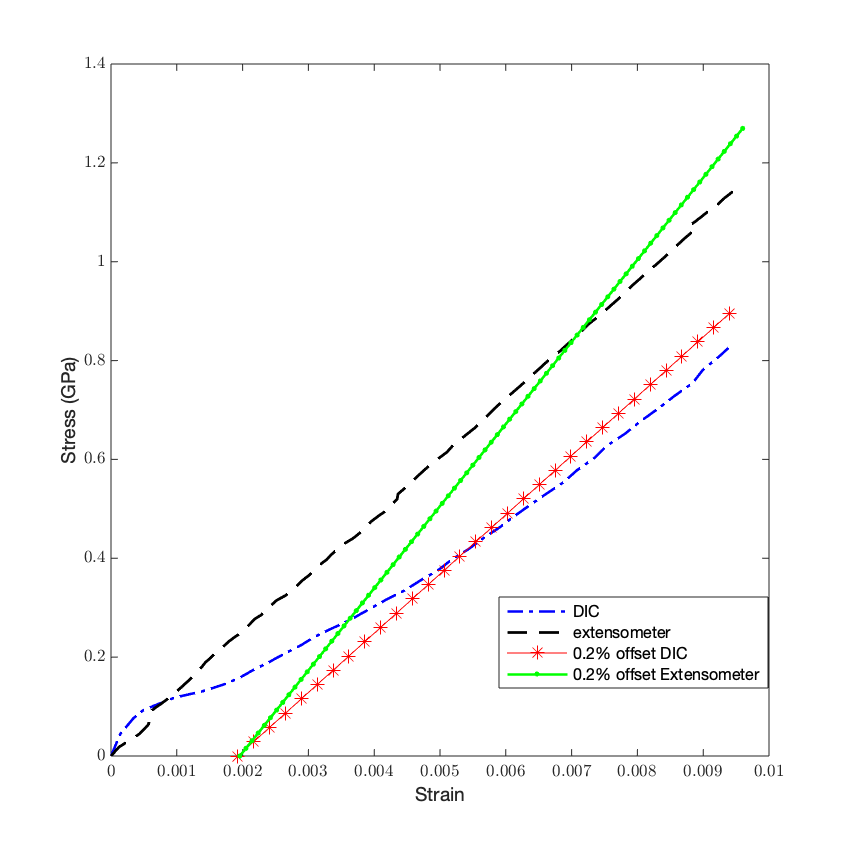
\includegraphics[width=\linewidth]{Pictures/stress vs strain/StressvsStrain_0.png}
        \caption{\textbf 0$\degree$ laminate}
        \label{fig:0lam}
    \end{subfigure}
    \begin{subfigure}[b]{0.45\linewidth}
        \centering
        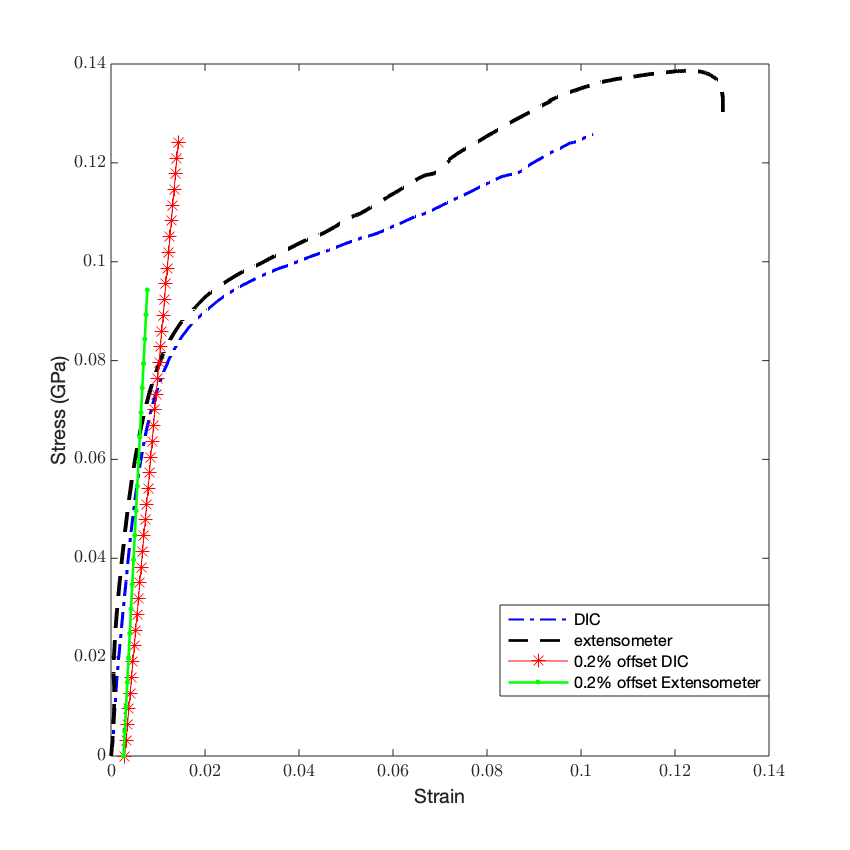
\includegraphics[width=\linewidth]{Pictures/stress vs strain/StressvsStrain_45.png}
        \caption{\textbf 45$\degree$ laminate}
        \label{fig:45lam}
    \end{subfigure}
    \end{center}
    \begin{center}
    \begin{subfigure}[b]{0.45\linewidth}
        \centering
        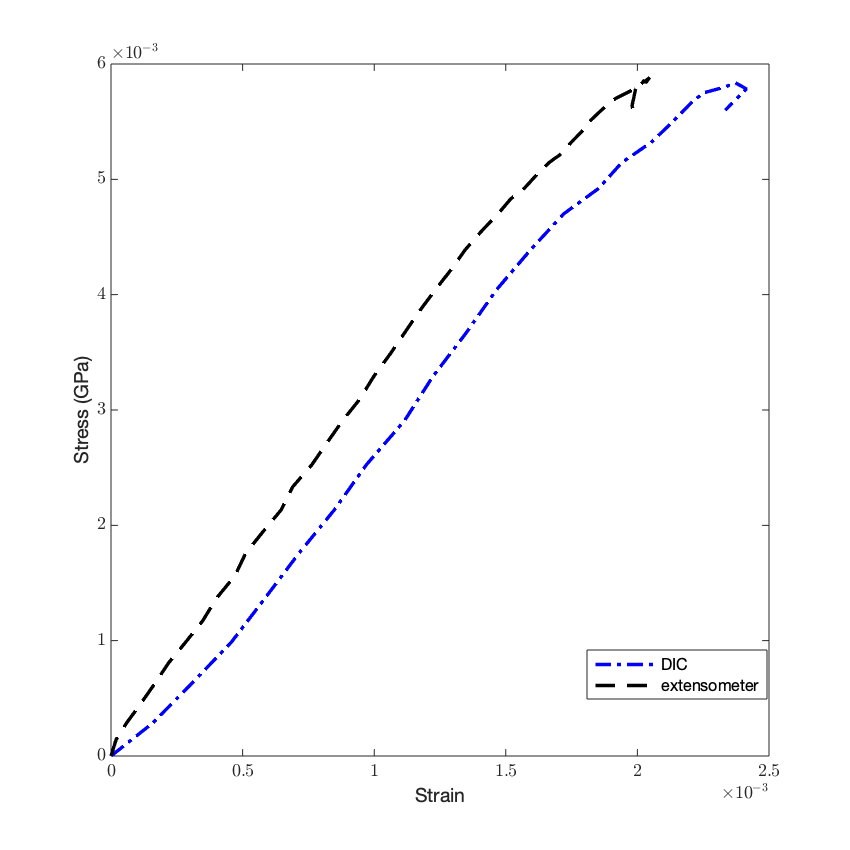
\includegraphics[width=\linewidth]{Pictures/stress vs strain/StressvsStrain_90.png}
        \caption{\textbf 90$\degree$ laminate}
        \label{fig:90lam}
    \end{subfigure}
    \end{center}
    \caption{Stress vs Strain plots comparing DIC to Extensometer measurements}
    \label{fig:stressvsstrain}
\end{figure}

\subsection{}
% Obtain experimental values of elastic modulus, elastic limit, ultimate strength, and ultimate strain for each specimen using the strain from the digital extensometer and the DIC calculations.  Tabulate all data and present them in your write-up.


\subsection{}
% Compute all on-axis and off-axis composite properties using the micromechanics models found in equations (6.8)-(6.11), (6.23)(6.27), and (6.28)-(6.33).
N

\subsection{}
% Compute the theoretical properties (E1, E2, nu12, and G6) for each composite specimen using equations (6.20) and (6.34)-(6.38).
N

\subsection{}
% Compare the experimental modulus (E1) for the composite specimens (as measured with the digital extensometer and from your DIC calculations) and the predictions determined in (4).

\begin{table}[!h]
    \centering
    \caption{Comparison of E$_{1}$ \cite{labmanual}}
    \begin{tabular}{|C{1in}|c|c|c|}\toprule
        \multicolumn{4}{c}{\textbf{Theoretical and Experimental Modulus}} \\ \midrule
        \textbf{Laminate\newline Orientation} & \textbf{Theoretical} & \textbf{DIC} & \textbf{Extensometer} \\ \hline\hline
         $0\degree$ & 130.37 GPa & 119.84 GPa & 166 GPa \\\hline
        $45\degree$ & 5.918 GPa & 10.9 GPa & 18 GPa  \\\hline
        $90\degree$ & 5.484 GPa & 2.69 GPa & 2.59 GPa \\\bottomrule
    \end{tabular}
    \label{tab:e1}
\end{table}

Compared to the theoretical values, the experimental modulus from DIC is lower for the $0\degree$ and $90\degree$ laminate orientations but greater for the $45\degree$ orientation. The experimental modulus from the extensometer is larger than the other results for both the $0\degree$ and $45\degree$ specimens but is the lowest for the $90\degree$ orientation.

\subsection{}
% Compute the theoretical failure loads of the 0 deg and 90 deg composite specimens using equation (6.54). Compute the failure load for the off-axis +/-45 deg composite specimen using the same equation (Hint: Assume theta = +45 deg only).  Compare these results with those obtained experimentally.
\begin{table}[!h]
    \centering
    \caption{Theoretical and Experimental Tensile Failure Loads \cite{labmanual}}
    \begin{tabular}{|C{1in}|c|c|}\toprule
        \multicolumn{3}{c}{\textbf{Tensile Failure Loads}} \\ \midrule
        \textbf{Laminate\newline Orientation} & \textbf{Theoretical} & \textbf{Experimental} \\ \hline\hline
        $0\degree$  & 1.930 GPa  & 1.156 GPa \\\hline
        $45\degree$ & 0.0668 GPa & 0.1386 GPa \\\hline
        $90\degree$ & 0.040 GPa  & 0.0059 GPa \\\bottomrule
    \end{tabular}
    \label{tab:failureloads}
\end{table}

The experimental failure loads are lower for the $0\degree$ and $90\degree$ laminate orientations. However, the experimental failure load is higher for the $45\degree$ specimen. 



\subsection{}
% Compute the specific elastic modulus and specific strength of all the specimens using the composite density data generated for each cured specimen in the manufacturing lab, Lab #1.  Compare the values of the three specimens to each another.
\begin{table}[!h]
    \centering
    \caption{Specimen specific properties \cite{labmanual}}
    \begin{tabular}{|C{1in}|c|c|}\toprule
        \multicolumn{3}{c}{\textbf{Specific Properties}} \\ \midrule
        \textbf{Laminate\newline Orientation} & \textbf{Specific Elastic Modulus} & \textbf{Specific Strength} \\ \hline\hline
         $0\degree$ & 76.21 MPa  & 735.1 $\frac{kPa}{kg/m^{3}}$ \\\hline
        $45\degree$ & 6.957 MPa & 88.49 $\frac{kPa}{kg/m^{3}}$  \\\hline
        $90\degree$ & 1.714 MPa & 3.749 $\frac{kPa}{kg/m^{3}}$  \\\bottomrule
    \end{tabular}
    \label{tab:specprop}
\end{table}

The specific elastic modulus and specific strength of the $0\degree$ laminate orientation specimen is much greater than the other two orientations. Even so, the $45\degree$ specimen still has significantly greater specific elastic modulus and specific strength than the $90\degree$ orientation.

\subsection{}
% Comment on any disparities between model predictions and experimental values.  What are possible causes of discrepancies? % ----

\clearpage
\section{Conclusions} \label{sec:7}
Composite materials have been investigated in this lab and were found to have properties that can be useful for aerospace applications. This lab has been broken down in two main experiments. The first portion of this lab was focused on the fabrication of multiple specimens of composites. Three different specimens with varying fiber directions were created. Based on pre published data sheets value, the fabricated specimens were reasonably on specification. Its densities, thickness, and fiber volumetric fractions were within 15\% of specification. However, its volumetric shrinkage percentage was significantly different, where a 70\% reduction was expected however only a 33\% reduction was observed. This could be attributed to imprecise manufacturing techniques resulting in excess material and voids in the composite. The second portion of the lab was focused on testing the performance of the specimens. Here, the effect of the fiber laminate angles becomes evident.  % ----


\clearpage
\label{sec:8}
\begin{thebibliography}{9}

\end{thebibliography}

\section{Contribution of Individual Group Members} \label{sec:9}
        \begin{table}[h!]
            \centering
            \begin{tabular}{|L{0.2\textwidth}|L{0.5\textwidth}|L{0.2\textwidth}|}
                \hline
                \multicolumn{3}{|c|}{\cellcolor{gray!50}\textbf{Team Member Contributions}} \\ \hline
                \cellcolor{gray!25}\textbf{Group Member} & \cellcolor{gray!25}\textbf{Contribution to Technical Report} & \cellcolor{gray!25}\textbf{UIN}\\ \hline
                Nicolas Alvarado &  & 79225\\\hline
                Kevin Chen \newline \textit{kevinjc2} &  & 02276\\\hline
                Joshua Clements &  & 35712\\ \hline
                Edward Guan &  &  14598 \\\hline
                Viraj Sampat &  & 25079\\\hline
            \end{tabular}
            \label{tab:contributions}
        \end{table}

\clearpage
\begin{alphasection}
    \section{SAMPLE CALCULATIONS}\label{sec:A}
    \setcounter{equation}{0}

\begin{enumerate}
    \item \textbf{Volume Fraction Calculation}
        \vspace{-0.25in}
        \begin{align*}
            \rho &= (\rho_{f})(V_{f}) + (\rho_{m})(1-V_{f}) \\
            1.4793 \frac{\text{g}}{\text{cm}^3} &= (1.84 \frac{\text{g}}{\text{cm}^3})(V_{f}) + (1.15 \frac{\text{g}}{\text{cm}^3})(1-V_{f}) \\
            V_{f} &= 0.4772
        \end{align*}
    \item \textbf{Volume Shrinkage Calculation}
        \vspace{-0.25in}
        \begin{align*}
            \% \text{Shrinkage} &= \frac{V_\text{uncured} - V_\text{cured}}{V_\text{cured}} * 100 \% \\
            &= \frac{11.65 \: \text{cm}^{3} - 8.74 \: \text{cm}^3}{8.74 \: \text{cm}^3} * 100 \% \\
            &= 33.28 \%
        \end{align*}
        
    % \item \textbf{ Next }
    %     \vspace{-0.25in}
    %     \begin{align*}
            
    %     \end{align*}

\end{enumerate}












% Template?
%  \setcounter{equation}{0}
%  \normalsize
%  \begin{enumerate}
%      \item \textbf{Buckling load of beam}\\
%         \begin{equation}
%              F = \frac{\pi E I_{y}}{lk^2}
%         \end{equation}
%         with, \\
%         lk = l = 0.65 m \\
%         E = $2.1 \times 10^{11} Pa$ \\
%         $I_{y} = 1.118 \times 10^{-10} m^4$ \\
%         \begin{equation}
%             F = \frac{\pi(2.1 \times 10^{11})(1.118 \times 10^{-10}) }{0.65^2} = 548.5 N
%         \end{equation}
% \end{enumerate}
    
    \section{ANALYSIS AND DERIVATIONS}\label{sec:B}
    \input{Sections/Appendix/AnalysisandDerivatives}
    
    \section{UNCERTAINTY ANALYSIS}\label{sec:C}
    To find the uncertainty, $U$, of the calculated variable, $f$, the following method of uncertainty propagation is used: 
\begin{align}
    U_{f} = \sqrt{(\frac{\delta f}{\delta x}U_{x})^{2} + (\frac{\delta f}{\delta x}U_{x})^{2}}
\end{align} \\
where $x$ and $y$ are variables present in the calculation of $f$. If $f$ is dependent on more variables, they are included in the equation identically to $x$ and $y$. \\

 \normalsize
 \begin{enumerate}
     \item \textbf{Specimen Volume}
     \vspace{-0.25in}
        \begin{align*}
        \text{Volume} &= \text{Length}*\text{Width}*\text{Thickness} \\
        \text{Length} &= 0.1689 m \text{ Width} = 0.02337 m \text{ Thickness} = 0.001549 m \\
        U_{V} &= \sqrt{(\frac{\delta V}{\delta l}U_{l})^{2} + (\frac{\delta V}{\delta w}U_{w})^{2}+(\frac{\delta V}{\delta t}U_{t})^{2}} \\
        U_{V} &= \sqrt{(w*t*U_{l})^{2} + (t*l*U_{w})^{2} + (w*l*U_{t})^{2} } \\ 
        U_{V} &= \sqrt{(w*t*0.00005)^{2} + (t*l*0.00000005)^{2} + (w*l*0.00000005)^{2} } \\ 
        U_{V} &= 0.0018 \text{ m}^{3} \\ 
        \end{align*}

\item \textbf{Specimen Density}
    \vspace{-0.25in}
    \begin{align*}
        \rho &= \frac{m}{V} \\ 
        U_{\rho} &= \sqrt{(\frac{\delta \rho}{\delta m}U_{m})^{2} + (\frac{\delta \rho}{\delta V}U_{V})^{2}} \\
        U_{\rho} &= \sqrt{(\frac{1}{V}U_{m})^{2} + (\frac{-m}{V^{2}}U_{V})^{2}} \\
        U_{\rho} &= 8.065 e -9 \quad kg/m^{3}
    \end{align*}

\end{enumerate}
    
    \section{RAW DATA} \label{sec:D}
    \begin{table}[!h]
    \centering
    \caption{Before Curing}
    \begin{tabular}{|l||c|c|c|c|}\toprule
        Specimen & Length \textit{(mm)} & Width \textit{(mm)} & Thickness \textit{(mm)} & Weight \textit{(g)} \\ \midrule
        \textbf{(a)}: $[90\degree]_{16\text{T}}$ & 174.1 & 25.4 & 2.635 & 17.15 \\\hline
        \textbf{(b)}: $[\pm45\degree_4]_{2\text{S}}$ & 172.4 & 25.4 & 3.299 & 21.17 \\\hline
        \textbf{(c)}: $[0\degree]_{8\text{T}}$ & 168.9 & 25.4 & 1.931 & 12.21 \\\bottomrule
    \end{tabular}
    \label{tab:beforedimensions}
\end{table}
\begin{table}[!h]
    \centering
    \caption{After Curing}
    \begin{tabular}{|l||c|c|c|c|}\toprule
        Specimen & Length \textit{(mm)} & Width \textit{(mm)} & Thickness \textit{(mm)} & Weight \textit{(g)} \\ \midrule
        \textbf{(a)}: $[90\degree]_{16\text{T}}$ & 174.1 & 22.70 & 2.213 & 13.72 \\\hline
        \textbf{(b)}: $[\pm45\degree_4]_{2\text{S}}$ & 172.4 & 24.74 & 2.535 & 16.94 \\\hline
        \textbf{(c)}: $[0\degree]_{8\text{T}}$ & 168.9 & 23.74 & 1.549 & 9.766 \\\bottomrule
    \end{tabular}
    \label{tab:afterdimensions}
\end{table}

\begin{table}[!h]
    \centering
    \caption{$0\degree$ Specimen (\textit{Trimmed Data})}
    \begin{tabular}{|c||c|c|c|}\toprule
        \textbf{Time (s)} & \textbf{Load} & \textbf{Strain (Ext)} & \textbf{Strain (DIC)}\\\midrule
        1 & 1640 & 0.0004 & 0.0001 \\\hline
        2 & 2825 & 0.0005 & 0.0003 \\\hline
        3 & 3397 & 0.0006 & 0.0004 \\\hline
        4 & 3882 & 0.0007 & 0.0007 \\\hline
        5 & 4351 & 0.0008 & 0.0009 \\\hline
        6 & 4823 & 0.0010 & 0.0013 \\\hline
        7 & 5331 & 0.0011 & 0.0017 \\\hline
        8 & 5859 & 0.0012 & 0.0019 \\\hline
        9 & 6404 & 0.0013 & 0.0021 \\\hline
        10 & 6987 & 0.0014 & 0.0024 \\\hline
        11 & 7580 & 0.0015 & 0.0026 \\\hline
        12 & 8206 & 0.0017 & 0.0028 \\\hline
        13 & 8858 & 0.0018 & 0.0030 \\\hline
        14 & 9509 & 0.0020 & 0.0033 \\\hline
        15 & 1016 & 0.0021 & 0.0036 \\\hline
        16 & 1086 & 0.0023 & 0.0039 \\\hline
        17 & 1158 & 0.0025 & 0.0041 \\\hline
        18 & 1231 & 0.0027 & 0.0044 \\\hline
        19 & 1306 & 0.0029 & 0.0047 \\\hline
        20 & 1382 & 0.0030 & 0.0049 \\\hline
        21 & 1460 & 0.0032 & 0.0051 \\\hline
        22 & 1538 & 0.0034 & 0.0054 \\\hline
        23 & 1618 & 0.0036 & 0.0056 \\\hline
        24 & 1700 & 0.0038 & 0.0059 \\\hline
        25 & 1784 & 0.0040 & 0.0061 \\\hline
        26 & 1869 & 0.0042 & 0.0063 \\\hline
        27 & 1948 & 0.0043 & 0.0066 \\\hline
        28 & 2036 & 0.0045 & 0.0068 \\\hline
        29 & 2125 & 0.0047 & 0.0070 \\\hline
        30 & 2216 & 0.0049 & 0.0073 \\\hline
        31 & 2305 & 0.0051 & 0.0075 \\\hline
        32 & 2397 & 0.0054 & 0.0078 \\\hline
        33 & 2490 & 0.0056 & 0.0080 \\\hline
        34 & 2584 & 0.0058 & 0.0083 \\\hline
        35 & 2679 & 0.0060 & 0.0085 \\\hline
        36 & 2774 & 0.0062 & 0.0088 \\\hline
        37 & 2870 & 0.0064 & 0.0089 \\\hline
        38 & 2967 & 0.0067 & 0.0092 \\\hline
        39 & 3064 & 0.0069 & 0.0094 \\\bottomrule
    \end{tabular}
    \label{tab:1}
\end{table}

\begin{table}[!h]
    \centering
    \caption{$45\degree$ Specimen (\textit{Trimmed Data})}
    \begin{tabular}{|c||c|c|c||c||c|c|c|}\toprule
        \textbf{Time (s)} & \textbf{Load} & \textbf{Strain (Ext)} & \textbf{Strain (DIC)} & \textbf{Time (s)} & \textbf{Load} & \textbf{Strain (Ext)} & \textbf{Strain (DIC)}\\\midrule
        1  & 163.93 & 0.0002 & 0.0004 & 41 & 4614 & 0.0082 & 0.0096 \\\hline
        2  & 500.78 & 0.0005 & 0.0007 & 42 & 4708 & 0.0086 & 0.0101 \\\hline
        3  & 707.28 & 0.0006 & 0.0009 & 43 & 4798 & 0.0091 & 0.0107 \\\hline
        4  & 858.38 & 0.0006 & 0.0011 & 44 & 4883 & 0.0096 & 0.0112 \\\hline
        5  & 965.23 & 0.0006 & 0.0012 & 45 & 4966 & 0.0101 & 0.0118 \\\hline
        6  & 1048 & 0.0005 & 0.0013 & 46 & 5043 & 0.0107 & 0.0123 \\\hline
        7  & 1142 & 0.0005 & 0.0014 & 47 & 5108 & 0.0111 & 0.0130 \\\hline
        8  & 1237 & 0.0006 & 0.0016 & 48 & 5177 & 0.0116 & 0.0136 \\\hline
        9  & 1337 & 0.0007 & 0.0017 & 49 & 5245 & 0.0122 & 0.0143 \\\hline
        10 & 1440 & 0.0007 & 0.0019 & 50 & 5313 & 0.0128 & 0.0149 \\\hline
        11 & 1538 & 0.0008 & 0.0021 & 51 & 5373 & 0.0135 & 0.0157 \\\hline
        12 & 1641 & 0.0010 & 0.0022 & 52 & 5431 & 0.0141 & 0.0164 \\\hline
        13 & 1744 & 0.0011 & 0.0024 & 53 & 5486 & 0.0147 & 0.0172 \\\hline
        14 & 1846 & 0.0012 & 0.0025 & 54 & 5537 & 0.0154 & 0.0180 \\\hline
        15 & 1946 & 0.0014 & 0.0027 & 55 & 5574 & 0.0160 & 0.0188 \\\hline
        16 & 2034 & 0.0015 & 0.0028 & 56 & 5615 & 0.0167 & 0.0195 \\\hline 
        17 & 2128 & 0.0017 & 0.0030 & 57 & 5654 & 0.0173 & 0.0203 \\\hline 
        18 & 2216 & 0.0018 & 0.0032 & 58 & 5694 & 0.0179 & 0.0211 \\\hline 
        19 & 2306 & 0.0020 & 0.0033 & 59 & 5735 & 0.0186 & 0.0219 \\\hline 
        20 & 2401 & 0.0021 & 0.0034 & 60 & 5776 & 0.0192 & 0.0227 \\\hline 
        21 & 2502 & 0.0023 & 0.0036 & 61 & 5813 & 0.0198 & 0.0236 \\\hline 
        22 & 2602 & 0.0025 & 0.0038 & 62 & 5848 & 0.0205 & 0.0244 \\\hline 
        23 & 2705 & 0.0027 & 0.0040 & 63 & 5880 & 0.0212 & 0.0253 \\\hline 
        24 & 2809 & 0.0029 & 0.0042 & 64 & 5912 & 0.0219 & 0.0261 \\\hline 
        25 & 2914 & 0.0031 & 0.0044 & 65 & 5943 & 0.0226 & 0.0271 \\\hline 
        26 & 3021 & 0.0033 & 0.0046 & 66 & 5973 & 0.0233 & 0.0279 \\\hline 
        27 & 3129 & 0.0035 & 0.0048 & 67 & 5999 & 0.0240 & 0.0289 \\\hline 
        28 & 3238 & 0.0038 & 0.0050 & 68 & 6028 & 0.0247 & 0.0297 \\\hline 
        29 & 3346 & 0.0040 & 0.0053 & 69 & 6055 & 0.0254 & 0.0307 \\\hline
        30 & 3458 & 0.0043 & 0.0055 & 70 & 6081 & 0.0262 & 0.0316 \\\hline
        31 & 3566 & 0.0045 & 0.0058 & 71 & 6108 & 0.0269 & 0.0326 \\\hline
        32 & 3676 & 0.0048 & 0.0061 & 72 & 6132 & 0.0277 & 0.0335 \\\hline
        33 & 3786 & 0.0051 & 0.0064 & 73 & 6156 & 0.0284 & 0.0345 \\\hline
        34 & 3893 & 0.0055 & 0.0067 & 74 & 6178 & 0.0291 & 0.0354 \\\hline
        35 & 4002 & 0.0058 & 0.0071 & 75 & 6198 & 0.0298 & 0.0364 \\\hline
        36 & 4110 & 0.0061 & 0.0074 & 76 & 6214 & 0.0306 & 0.0372 \\\hline
        37 & 4215 & 0.0065 & 0.0078 & 77 & 6235 & 0.0313 & 0.0382 \\\hline
        38 & 4318 & 0.0069 & 0.0082 & 78 & 6257 & 0.0321 & 0.0390 \\\hline
        39 & 4420 & 0.0073 & 0.0086 & 79 & 6279 & 0.0328 & 0.0400 \\\hline
        40 & 4519 & 0.0077 & 0.0091 & 80 & 6301 & 0.0334 & 0.0409 \\\hline
    \end{tabular}
    \label{tab:2}
\end{table}


\begin{table}[!h]
    \centering
    \caption{$45\degree$ Specimen (\textit{Trimmed Data (continued)})}
    \begin{tabular}{|c||c|c|c||c||c|c|c|}\toprule
        \textbf{Time (s)} & \textbf{Load} & \textbf{Strain (Ext)} & \textbf{Strain (DIC)} & \textbf{Time (s)} & \textbf{Load} & \textbf{Strain (Ext)} & \textbf{Strain (DIC)}\\\midrule
        81 & 6321 & 0.0341 & 0.0418  & 121 & 7094 & 0.0589 & 0.0743 \\\hline
        82 & 6343 & 0.0348 & 0.0427  & 122 & 7118 & 0.0596 & 0.0751 \\\hline
        83 & 6362 & 0.0354 & 0.0436  & 123 & 7140 & 0.0602 & 0.0759 \\\hline
        84 & 6380 & 0.0361 & 0.0445  & 124 & 7161 & 0.0608 & 0.0765 \\\hline
        85 & 6401 & 0.0367 & 0.0455  & 125 & 7183 & 0.0614 & 0.0773 \\\hline
        86 & 6416 & 0.0371 & 0.0463  & 126 & 7207 & 0.0620 & 0.0780 \\\hline
        87 & 6438 & 0.0378 & 0.0472  & 127 & 7229 & 0.0626 & 0.0788 \\\hline
        88 & 6459 & 0.0385 & 0.0481  & 128 & 7251 & 0.0632 & 0.0796 \\\hline
        89 & 6480 & 0.0392 & 0.0490  & 129 & 7272 & 0.0638 & 0.0804 \\\hline
        90 & 6502 & 0.0399 & 0.0499  & 130 & 7293 & 0.0644 & 0.0810 \\\hline
        91 & 6520 & 0.0406 & 0.0508  & 131 & 7315 & 0.0650 & 0.0818 \\\hline
        92 & 6538 & 0.0413 & 0.0516  & 132 & 7337 & 0.0657 & 0.0825 \\\hline
        93 & 6557 & 0.0419 & 0.0526  & 133 & 7356 & 0.0663 & 0.0833 \\\hline
        94 & 6577 & 0.0425 & 0.0534  & 134 & 7361 & 0.0666 & 0.0840 \\\hline
        95 & 6593 & 0.0432 & 0.0543  & 135 & 7375 & 0.0673 & 0.0847 \\\hline
        96 & 6599 & 0.0439 & 0.0550  & 136 & 7379 & 0.0679 & 0.0853 \\\hline
        97 & 6616 & 0.0445 & 0.0559  & 137 & 7387 & 0.0684 & 0.0860 \\\hline
        98 & 6633 & 0.0451 & 0.0566  & 138 & 7398 & 0.0690 & 0.0865 \\\hline
        99 & 6653 & 0.0458 & 0.0575  & 139 & 7419 & 0.0695 & 0.0872 \\\hline
        100 & 6673 & 0.0464 & 0.0582 & 140 & 7448 & 0.0700 & 0.0878  \\\hline
        101 & 6695 & 0.0470 & 0.0591 & 141 & 7478 & 0.0706 & 0.0885  \\\hline
        102 & 6716 & 0.0476 & 0.0598 & 142 & 7506 & 0.0711 & 0.0892  \\\hline
        103 & 6737 & 0.0483 & 0.0606 & 143 & 7532 & 0.0716 & 0.0899  \\\hline
        104 & 6752 & 0.0486 & 0.0614 & 144 & 7555 & 0.0721 & 0.0906  \\\hline
        105 & 6776 & 0.0492 & 0.0622 & 145 & 7577 & 0.0721 & 0.0913  \\\hline
        106 & 6798 & 0.0499 & 0.0630 & 146 & 7603 & 0.0727 & 0.0920  \\\hline
        107 & 6819 & 0.0505 & 0.0638 & 147 & 7627 & 0.0733 & 0.0927  \\\hline
        108 & 6839 & 0.0512 & 0.0645 & 148 & 7651 & 0.07393 & 0.0934 \\\hline
        109 & 6858 & 0.0518 & 0.0654 & 149 & 7672 & 0.07450 & 0.0941 \\\hline
        110 & 6868 & 0.0525 & 0.0661 & 150 & 7693 & 0.07506 & 0.0948 \\\hline
        111 & 6885 & 0.0531 & 0.0669 & 151 & 7713 & 0.07562 & 0.0957 \\\hline
        112 & 6905 & 0.0537 & 0.0676 & 152 & 7735 & 0.07616 & 0.0963 \\\hline
        113 & 6925 & 0.0543 & 0.0684 & 153 & 7758 & 0.07671 & 0.0971 \\\hline
        114 & 6948 & 0.0549 & 0.0690 & 154 & 7779 & 0.07728 & 0.0977 \\\hline
        115 & 6970 & 0.0555 & 0.0698 & 155 & 7781 & 0.07769 & 0.0984 \\\hline
        116 & 6992 & 0.0561 & 0.0705 & 156 & 7796 & 0.07818 & 0.0991 \\\hline
        117 & 7015 & 0.0567 & 0.0714 & 157 & 7816 & 0.07868 & 0.0998 \\\hline
        118 & 7037 & 0.0573 & 0.0721 & 158 & 7835 & 0.07920 & 0.1004 \\\hline
        119 & 7058 & 0.0579 & 0.0729 & 159 & 7855 & 0.07973 & 0.1012 \\\hline
        120 & 7078 & 0.0585 & 0.0736 & 160 & 7874 & 0.08028 & 0.1018 \\\bottomrule
    \end{tabular}
    \label{tab:3}
\end{table}


\begin{table}[!h]
    \centering
    \caption{$90\degree$ Specimen (\textit{Trimmed Data})}
    \begin{tabular}{|c||c|c|c|}\toprule
        \textbf{Time (s)} & \textbf{Load} & \textbf{Strain (Ext)} & \textbf{Strain (DIC)}\\\midrule
        1 & 14.36 & 5.909e-05  & 0.0001 \\\hline
        2 & 31.43 & 0.0001 & 0.0003 \\\hline
        3 & 49.62 & 0.0002 & 0.0004 \\\hline
        4 & 68.88 & 0.0004 & 0.0005 \\\hline
        5 & 88.23 & 0.0005 & 0.0007 \\\hline
        6 & 107.1 & 0.0006 & 0.0008 \\\hline
        7 & 126.7 & 0.0007 & 0.0009 \\\hline
        8 & 146.0 & 0.0008 & 0.0011 \\\hline
        9 & 165.1 & 0.0009 & 0.0012 \\\hline
        10 & 183.8 & 0.0011 & 0.0013 \\\hline
        11 & 202.9 & 0.0012 & 0.0014 \\\hline
        12 & 220.3 & 0.0013 & 0.0015 \\\hline
        13 & 236.1 & 0.0014 & 0.0017 \\\hline
        14 & 247.1 & 0.0015 & 0.0018 \\\hline
        15 & 258.3 & 0.0016 & 0.0019 \\\hline
        16 & 267.2 & 0.0017 & 0.0020 \\\hline
        17 & 275.8 & 0.0018 & 0.0021 \\\hline
        18 & 284.9 & 0.0018 & 0.0022 \\\hline
        19 & 288.8 & 0.0019 & 0.0022 \\\hline
        20 & 291.2 & 0.0020 & 0.0023 \\\hline
        21 & 293.1 & 0.0020 & 0.0023 \\\hline
        22 & 290.4 & 0.0019 & 0.0024 \\\hline
        23 & 281.2 & 0.0019 & 0.0023 \\\hline
        24 & 233.3 & 0.0012 & 0.0022 \\\hline
        25 & 221.4 & 0.0010 & 0.0020 \\\hline
        26 & 215.2 & 0.0010 & 0.0020 \\\hline
        27 & 202.1 & 0.0010 & 0.0020 \\\hline
        28 & 175.8 & 0.0007 & 0.0020 \\\hline
        29 & 109.3 & 0.0002 & 0.0016 \\\hline
        30 & 80.43 & 8.863e-05 & 0.0017 \\\hline
        31 & 79.25 & 6.894e-05 & 0.0017 \\\hline
        32 & 74.41 & 1.969e-05 & 0.0017 \\\hline
        33 & 72.93 & 1.969e-05 & 0.0017 \\\hline
        34 & 74.11 & 0 & 0.0059 \\\hline
        35 & 65.72 & -4.924e-05 & 0.0017 \\\bottomrule
    \end{tabular}
    \label{tab:4}
\end{table}
    
\end{alphasection}

% \newpage


% \hspace{-0.5in}\large{\textbf{APPENDIX A: SAMPLE CALCULATIONS}} \label{sec:A} 
% \normalsize

% \clearpage
% \hspace{-0.5in}\large{\textbf{APPENDIX B: ANALYSIS AND DERIVATIONS}} \label{sec:B} \\ 
% \normalsize


% \clearpage


% \hspace{-0.5in}\large{\textbf{APPENDIX C: UNCERTAINTY ANALYSIS}} \label{sec:C} 
% \normalsize



% \clearpage
% \hspace{-0.5in}\large{\textbf{APPENDIX D: RAW DATA}} \label{sec:D}
% \\

% \clearpage
% \hspace{-0.5in}\large{\textbf{APPENDIX E: GROUP MEMBER CONTRIBUTIONS}} \label{sec:E}
% \begin{table}[h!]
%     \centering
%     \begin{tabular}{|C{0.2\textwidth}|C{0.5\textwidth}|}
%         \hline
%         \multicolumn{2}{|c|}{\cellcolor{gray!25}\textbf{Team Member Contributions}} \\ \hline
%         \cellcolor{gray!25}\textbf{Group Member} & \cellcolor{gray!25}\textbf{Contribution to Technical Report} \\ \hline
%         & \\\hline
%         & \\\hline
%         & \\\hline
%         & \\\hline
%     \end{tabular}
%     \caption{Individual Tasks Completed per Member}
%     \label{tab:contributions}
% \end{table}



\newpage





\end{document}
